\documentclass[a4paper, 12pt, oneside]{article}
 
\usepackage[german]{babel}
\usepackage[utf8]{inputenc}
\usepackage[T1]{fontenc}
\usepackage{ae}
\usepackage[table]{xcolor}
%\usepackage[bookmarks,bookmarksnumbered]{hyperref}
\usepackage{graphics}
\usepackage{wrapfig}
\usepackage{amsmath}           %macht
\usepackage{amsfonts}          %       Mathe
\usepackage{amssymb}           %              mächtiger
\usepackage{graphicx}          %erlaubt Graphiken einzubinden (.eps für dvi und ps sowie .jpg für pdf)
\usepackage[T1]{fontenc}       %Zeichenbelegung der verwendeten Schrift
\usepackage{typearea}	         %ermöglicht änderung des Seitenspiegels
\usepackage{lastpage}          %lässt auf die Seienanzahl zugreifen
\usepackage[margin=10pt,font=small,labelfont=bf]{caption} %macht die Bildbeschriftungen richtig
\usepackage{microtype}
\usepackage{bm}               % bold math, für \bm{}
\usepackage{enumerate}        % verbessert Aufzählungen
\usepackage{array}            % für Tabellen: bindet tabular-Umgebung ein
\usepackage{pdfpages}         % für die Einbindung kompletter pdf-*Seiten*
\usepackage{parskip}          % zw. Absätzen: eine knappe Leerzeile statt hängender Einzüge
\usepackage{dsfont}
\usepackage{tocloft}			% Manipulation des Inhaltsverzeichnisses
\usepackage{siunitx}
\usepackage{parskip}
\usepackage{multirow}
\usepackage{wasysym}
\usepackage{float}
\usepackage{slantsc}
\usepackage{parskip}          % zw. Absätzen: eine knappe Leerzeile statt hängender Einzüge
\usepackage{blindtext}

%%%%%%%%%%%%%%%%%%%%%%%%%%%%%%%%%%%%%%%%%%%%%%%%%%%%%%%%%%%%%%%%%%%%%%%%%%%%%%
%	Abbildungen werden mit Abb. angezeigt.
%
\addto\captionsgerman{%
  \renewcommand{\figurename}{Abb.}%
  \renewcommand{\tablename}{Tab.}%
} 
%
%%%%%%%%%%%%%%%%%%%%%%%%%%%%%%%%%%%%%%%%%%%%%%%%%%%%%%%%%%%%%%%%%%%%%%%%%%%%%%


%%%%%%%%%%%%%%%%%%%%%%%%%%%%%%%%%%%%%%%%%%%%%%%%%%%%%%%%%%%%%%%%%%%%%%%%%%%%%%
%	Kopf- und Fussleiste.
%
\usepackage{fancyhdr}
\fancyhead[LO,LE]{Dokumentation -- 3D-Modellierung und Animation}
\fancyhead[CO,CE]{}
%\fancyhead[RO,RE]{\rightmark}
\fancyfoot[LO,LE]{}

\fancyfoot[CO,CE]{}
\fancyfoot[RO,RE]{\thepage}
%
%%%%%%%%%%%%%%%%%%%%%%%%%%%%%%%%%%%%%%%%%%%%%%%%%%%%%%%%%%%%%%%%%%%%%%%%%%%%%%
 
%%%%%%%%%%%%%%%%%%%%%%%%%%%%%%%%%%%%%%%%%%%%%%%%%%%%%%%%%%%%%%%%%%%%%%%%%%%%%%
%
% Größenanpassungen
%


\usepackage[a4paper]{geometry}
\usepackage{setspace}
\setlength{\unitlength}{1cm}
\setlength{\oddsidemargin}{0.8cm}
\setlength{\evensidemargin}{-0.3cm}
\setlength{\textwidth}{15.5cm}
\setlength{\topmargin}{-1cm}
\setlength{\textheight}{23cm}
\columnsep 0.5cm
\setstretch{1.15} 
%
%%%%%%%%%%%%%%%%%%%%%%%%%%%%%%%%%%%%%%%%%%%%%%%%%%%%%%%%%%%%%%%%%%%%%%%%%%%%%% 
 
\begin{document}
  
	\begin{titlepage}
		
		\begin{center}
			~\\[0cm]
			Berufsakademie Sachsen \\
			Staatliche Studienakadamie Leipzig \\[2.0cm]
			
			\begin{huge}
				\textbf{Dokumentation über die Erstellung einer Landschaft mit Unity und \\3D Studio Max} \\[2.4cm]
			\end{huge}
			
			\doublespacing
			
			Helms Klamm\\
			3D-Modellierung und Animation\\ 
			6. Semester \\[3.0cm]
		\end{center}
		
		\onehalfspacing
		\begin{tabbing}
			Eingereicht von:  \= ~ \= ~ \= Daniel Gilgen \= ~ \= ~ \= ~ \= ~ \= ~ \= ~ \= ~ \= ~ \= ~ \= Ronny Zingler \\
			  \> \> \> Straße des 18. Okt. 31 	\> \> \> \> \> \> \> \> \> \> Kochstraße 20 \\
			  \> \> \> 04103 Leipzig \> \> \> \> \> \> \> \> \> \>  04275  Leipzig \\
			  \> \> \> CS14-01 	\> \> \> \> \> \> \> \> \> \>  CS14-01 \\
			  \> \> \> 5000616 \> \> \> \> \> \> \> \> \> \>  5000568 \\
			\\
			Dozent:  \> \> \> Prof. Vyhnal \\
		\end{tabbing}
		\vspace*{\fill}
		Leipzig, \today
		
	\end{titlepage}
 
 
% Platzierung des Inhaltsverzeichnisses
\newpage
\tableofcontents
\pagestyle{fancy}

\newpage 
\section{Einleitung (Grundlage, Vorüberlegung ..)}

Die Thematik des 3D-Modellierungs- und Animationsprojekt ist eine fiktive Welt, angelehnt an die Belagerung Helms Klamms. Es handelt sich darin um eine Szene aus dem Film Herr der Ringe: Die zwei Türme. Helms Klamm ist eine massive Befestigungsanlage am Fuße eines Berges. Vor Beginn der eigentlichen Arbeiten mussten Vorüberlegungen gemacht werden, in welchen die Grundzüge der 3D-Szene festgelegt wurden. In Abb.\ref{handskizze} sieht man die ersten Entwürfe in Form von Handskizzen. Die linke Skizze zeigt die grobe Aufteilung der Szene und rechts ist ein Grobentwurf der Burg zu sehen.

\begin{figure}[h]
	
	\centering
	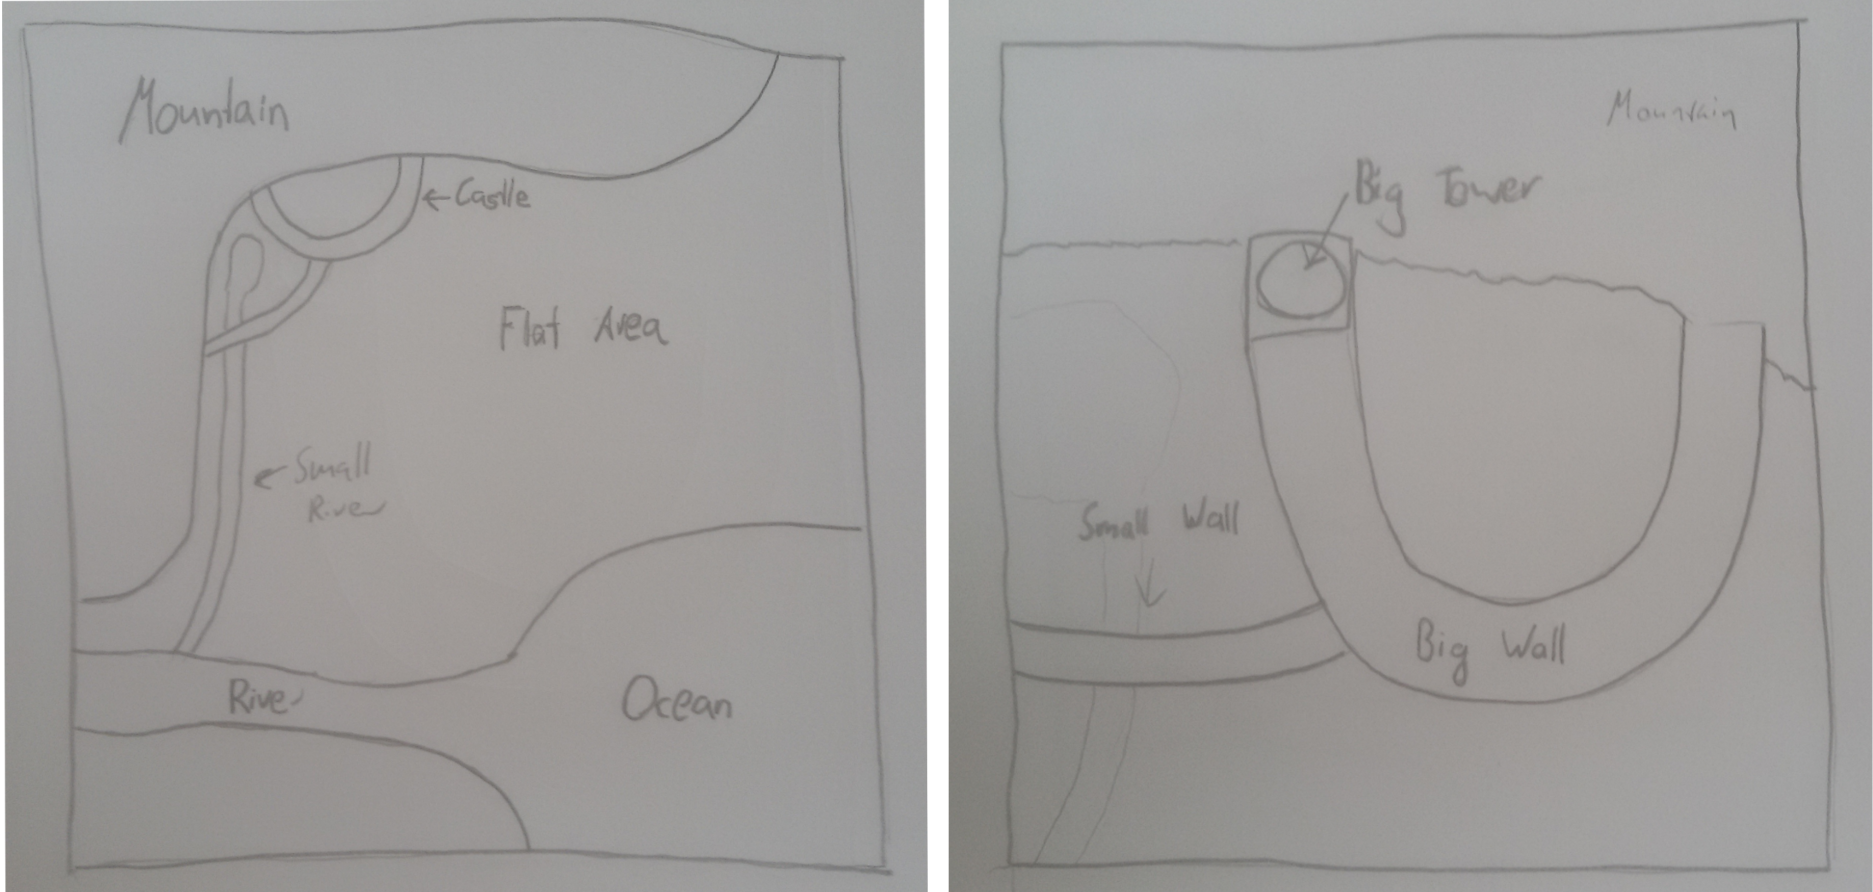
\includegraphics[width=0.95\linewidth]{Abbildungen/Unity/Skizzen}
	\caption{Handskizzen als Vorüberlegung}
	\label{handskizze}
\end{figure}


Die Größen wurden so festgelegt, dass sie begehbar ist und einen massiven Eindruck hinterlässt. Gesetze der realen Welt spielten beim Entwurf der Burg keine Rolle. Auf Grundlage der gemeinsamen Überlegungen wurden die Abmessungen der Festung festgelegt und ein erstes Modell erstellt. Dieses war die Basis der gemeinsamen Projektarbeit und ermöglichte ein paralleles Arbeiten in Unity und 3d Studio Max.

Im Verlaufe der Arbeit wurden die beiden Teile immer wieder abgeglichen, Details hinzugefügt, das weitere Vorgehen besprochen und sukzessive entstand so die finale Szene. 
\newpage
\section{Modellierung mit Unity}

\subsection{Gelände}
\begin{figure}[h]
\centering
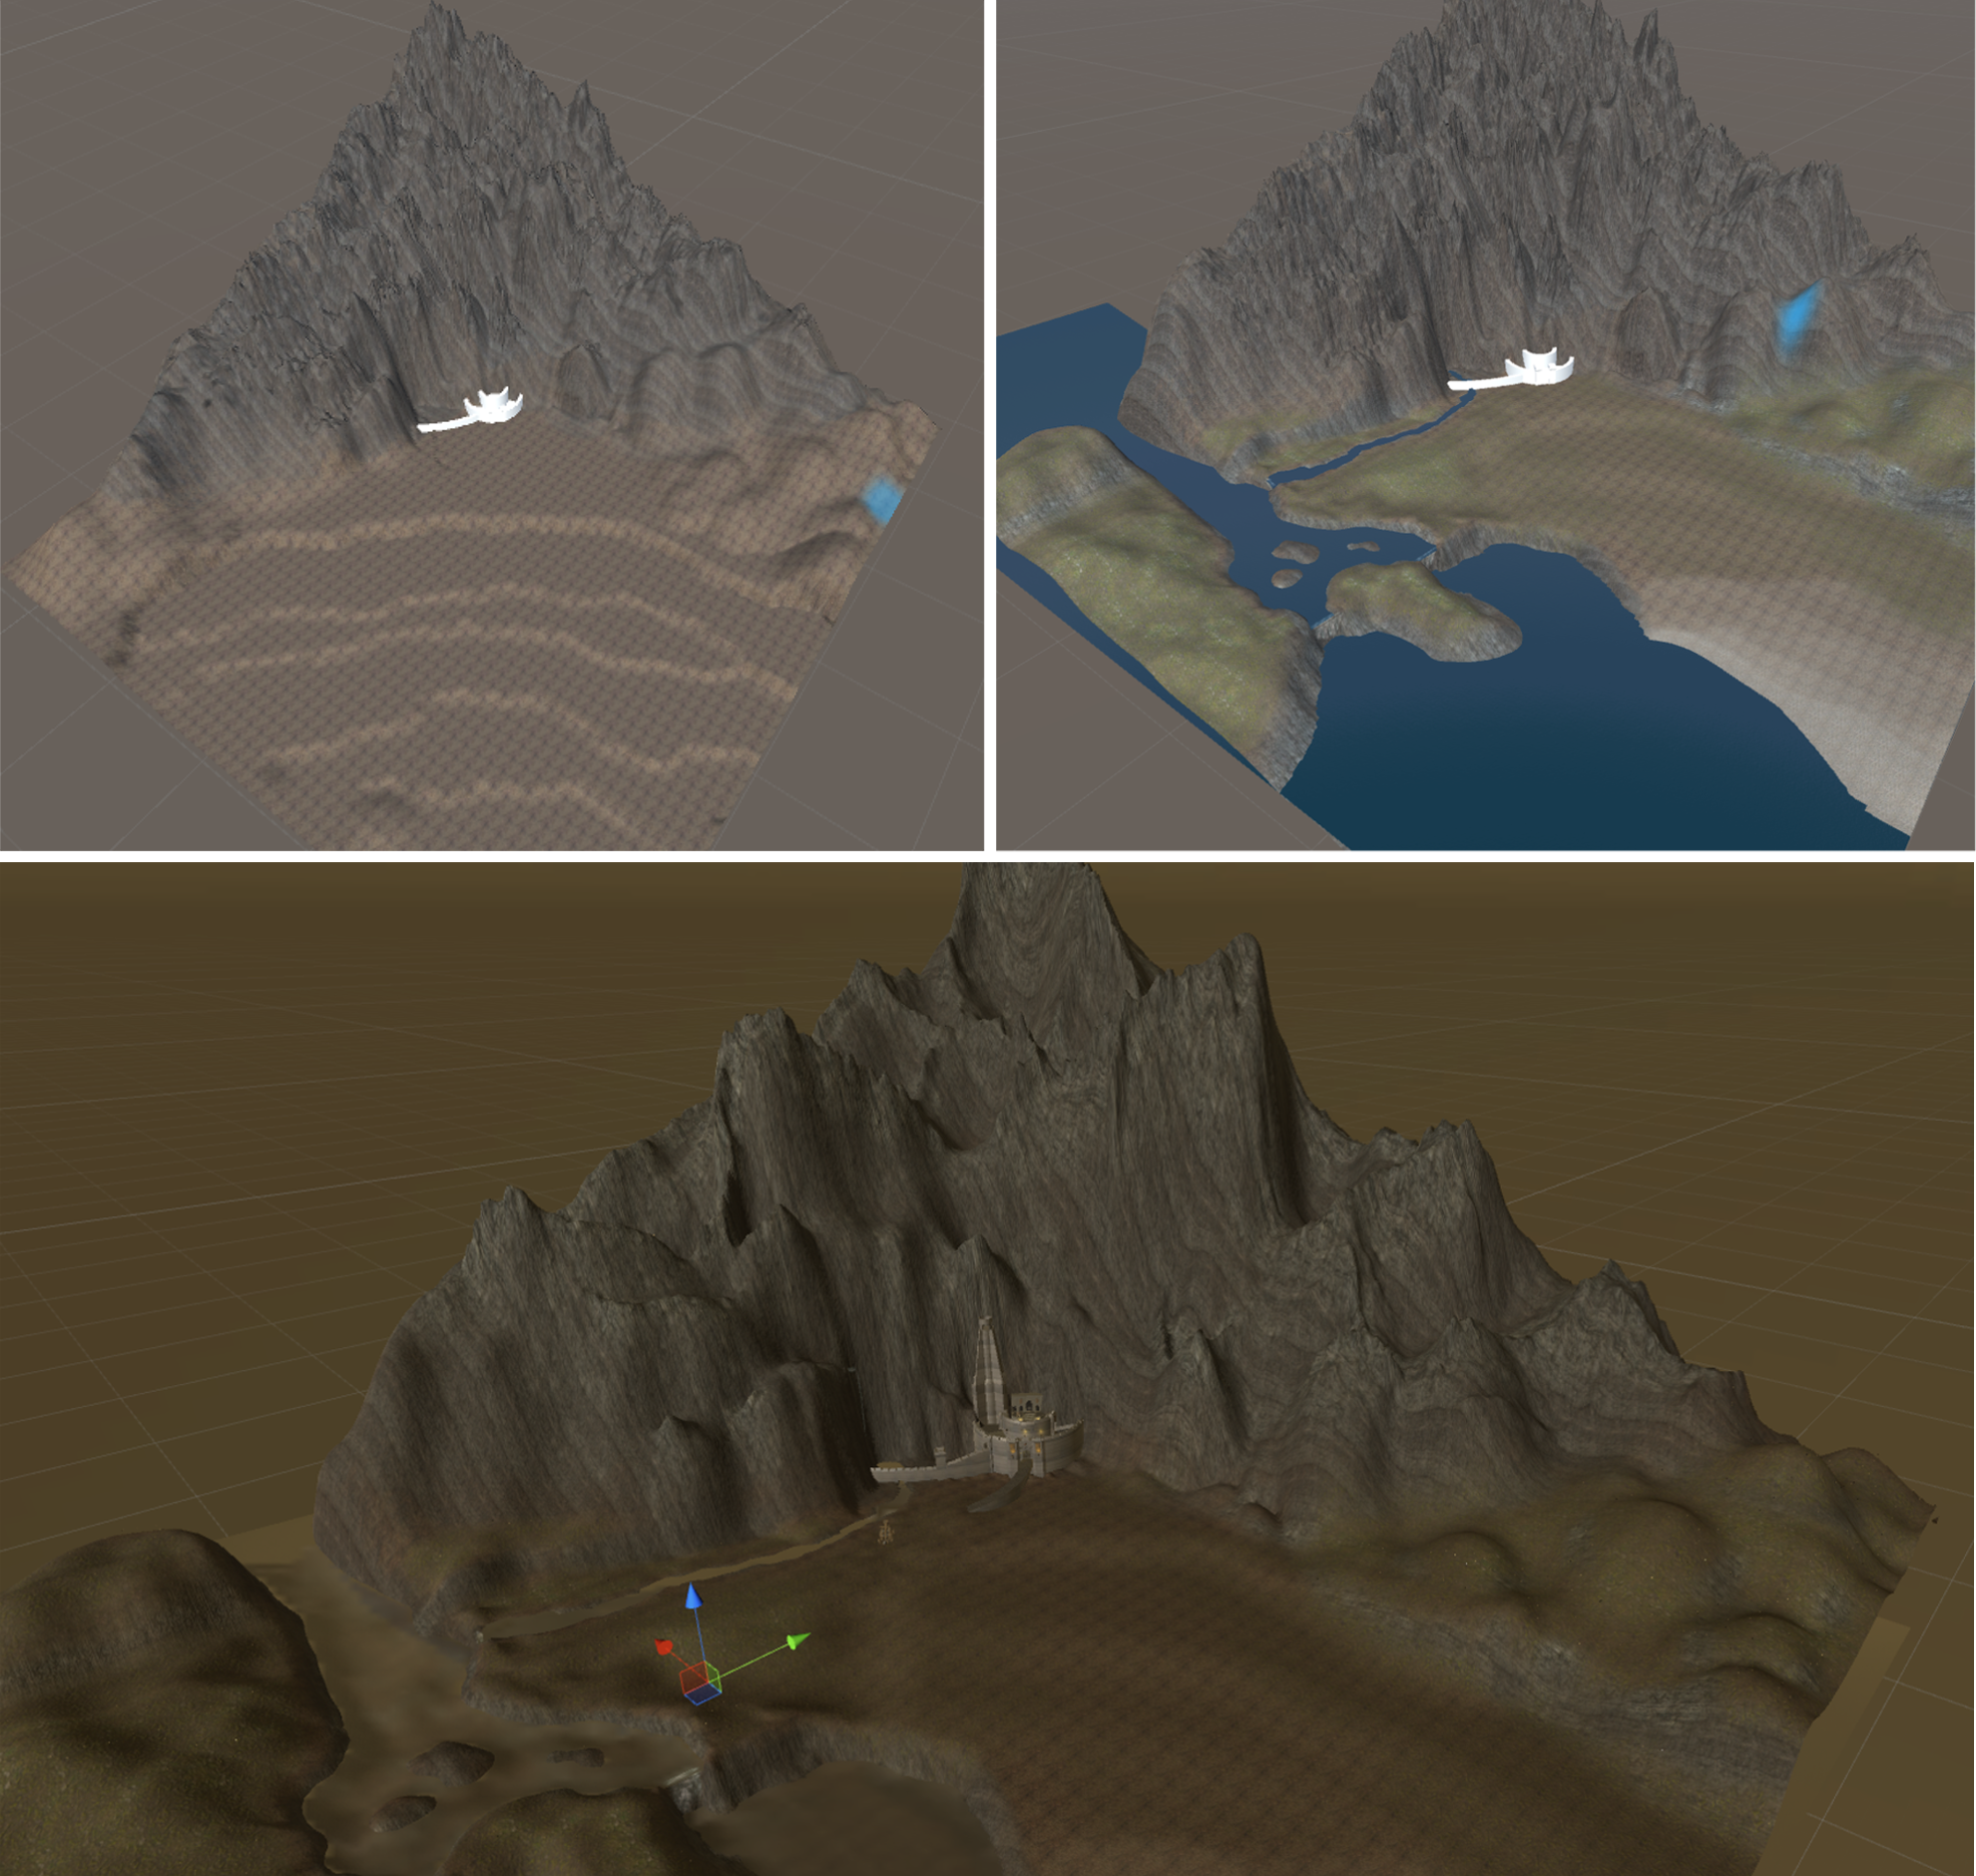
\includegraphics[width=0.95\linewidth]{Abbildungen/Unity/TerrainProgress}
\caption{Entwicklungsschritte des Geländes}
\label{fig:TerrainProgress}
\end{figure}

\begin{wrapfigure}[8]{r}{0.5\textwidth}
	\vspace{-20pt}
	\begin{center}
		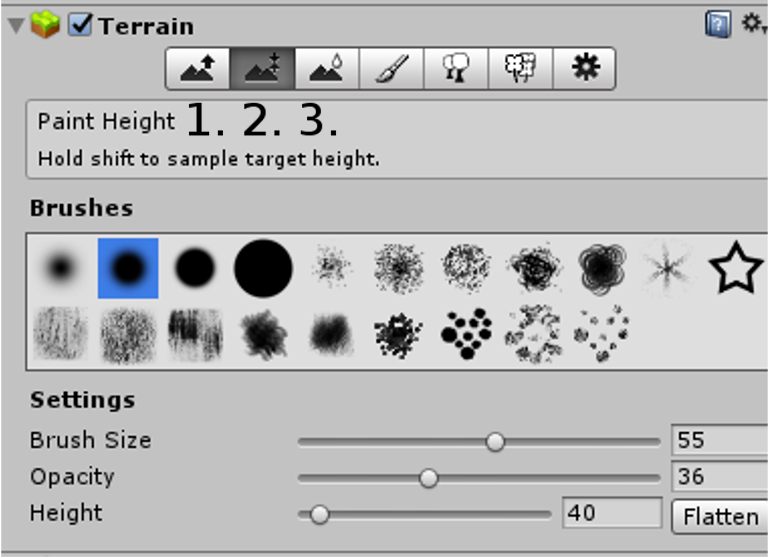
\includegraphics[width=0.45\textwidth]{Abbildungen/Unity/TerrainTool}
	\end{center}
	\caption{Terrain Werkzeuge}
	\label{fig:TerrainWerkzeuge}
\end{wrapfigure}

Die Abb. \ref{fig:TerrainProgress} zeigt verschieden Zwischenstände in der Gestaltung des Geländes. Die genutzten Werkzeuge sind in Abb. \ref{fig:TerrainWerkzeuge}, namentlich \textit{Raise/Lower} (1.), \textit{Paint Height} (2.) und \textit{Smooth Height} (3.), zu sehen. In allen drei Werkzeugen stehen verschieden Einstellungen für die Weite und Deckkraft des Pinsels zur Verfügung. Das Werkzeug \textit{Raise/Lower} ist besonders empfindlich und deshalb sollten für dieses nur niedrige Deckkraftwerte eingestellt werden.

%\newpage
Um ein gutes Größenverhältnis zwischen Burg und Gelände zu erreichen wurden die Maße des Terrains auf 500*500*600 festgelegt. Die Starthöhe des Geländes wurde mittels \textit{Paint Height} und \textit{Flatten} auf 50m gesetzt und von diesem Punkt heraus wurden die anderen Teile Stück für Stück herausgearbeitet. Mittel der Wahl war eine Kombination aus \textit{Paint Height} und \textit{Smooth Height}, gut zu sehen links oben in Abb. \ref{fig:TerrainProgress}. Zuerst wurde terrassenförmig die Höhe herausgearbeitet und danach wieder geglättet, um für fließende Übergänge zu sorgen. Das Gebirge im Hintergrund wurde größtenteils mit \textit{Raise/Lower} gestaltet. Es unterlag allerdings im Designprozess vielen Änderungen, da die Wirkung aus der Ego-Perspektive und das Zusammenspiel mit der Festung nicht optimal war. Im unteren Teil der Abb. \ref{fig:TerrainProgress} ist der finale Zustand des Geländes zu sehen.

\subsection{Texturierung}
\begin{figure}[h]
	\centering
	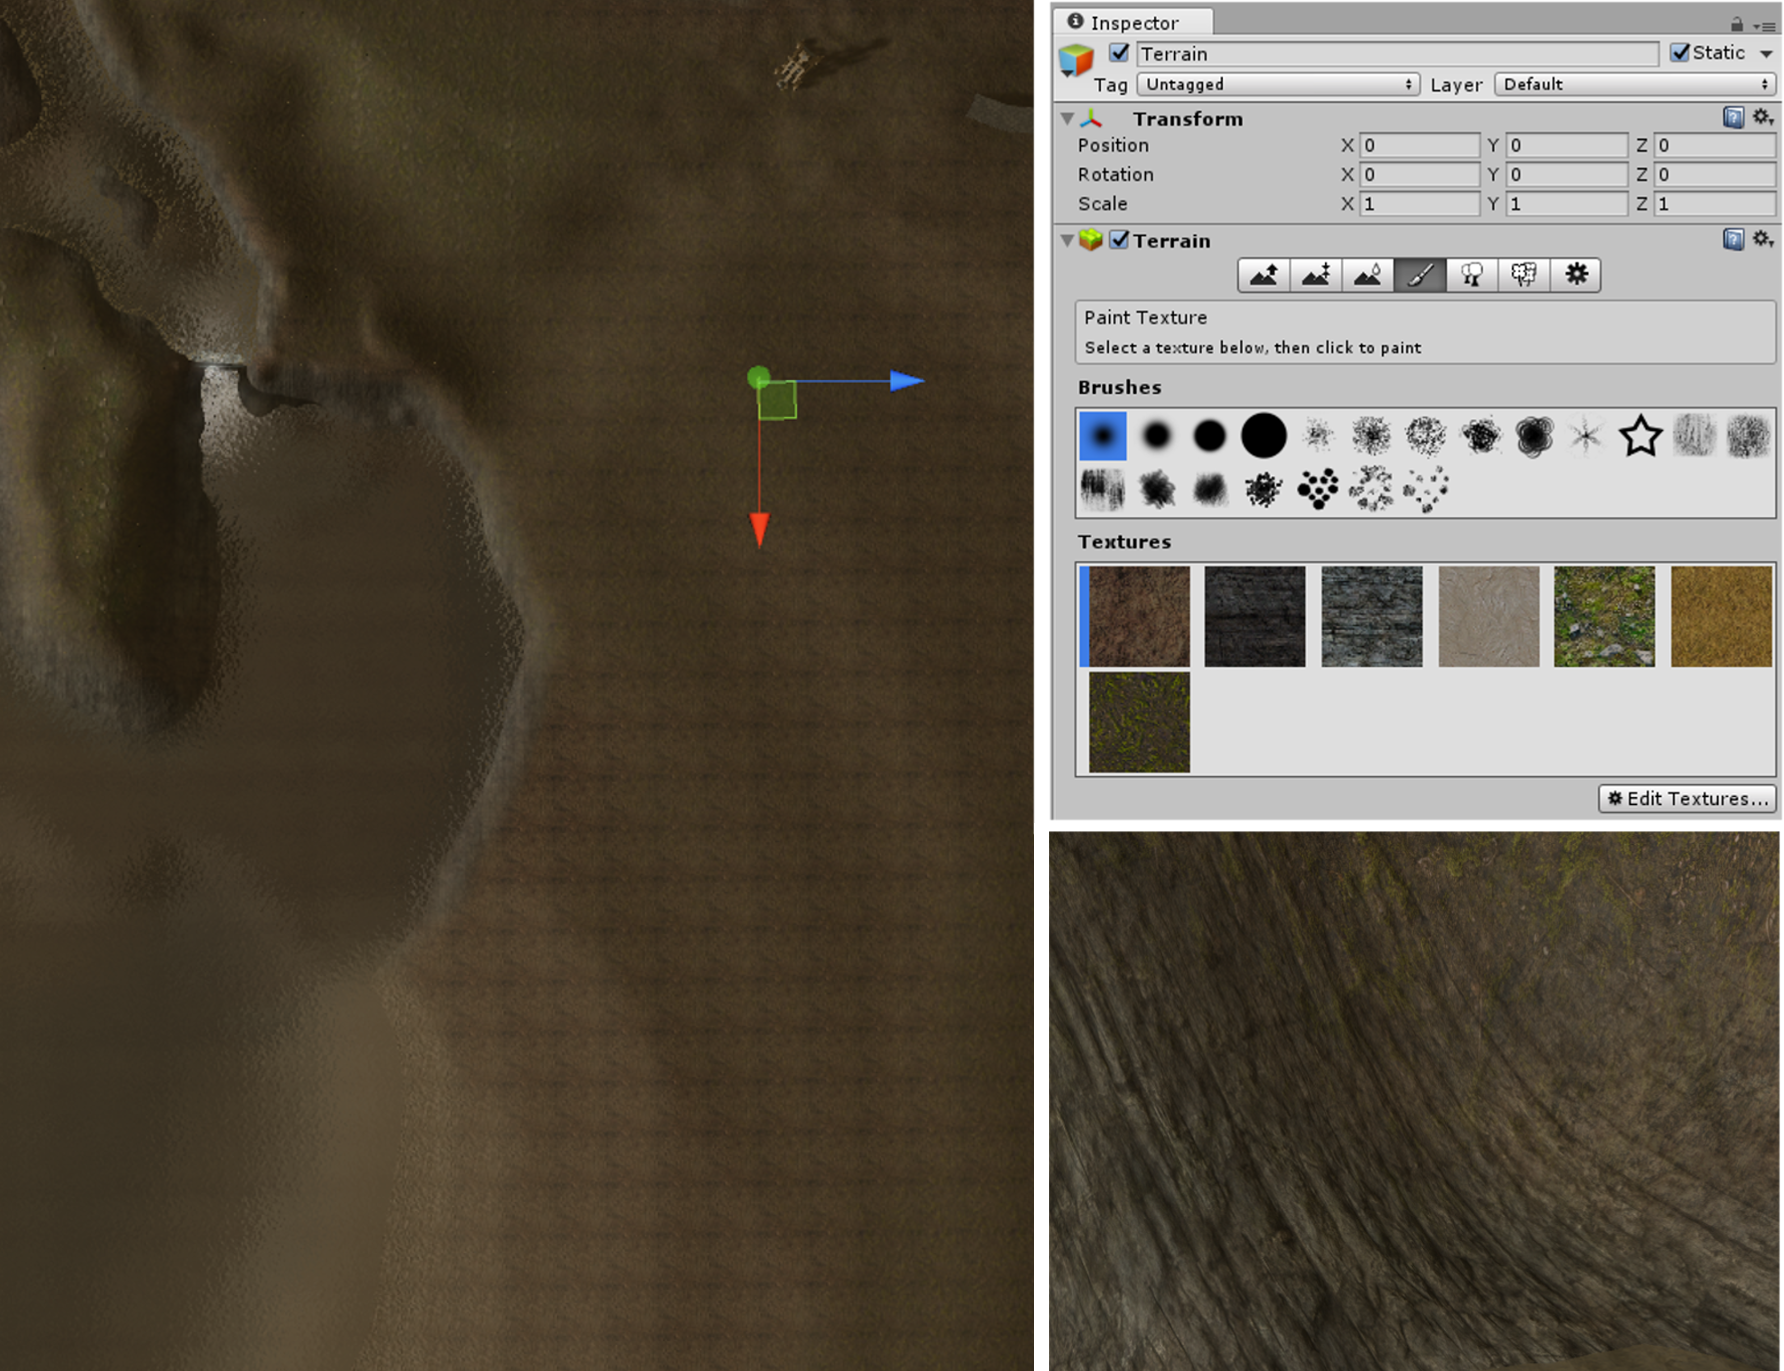
\includegraphics[width=0.95\linewidth]{Abbildungen/Unity/Texture}
	\caption{Wasserebenen und exemplarische Einstellungen}
	\label{fig:Textures}
\end{figure}

Das Gelände mit Texturen zu versehen ist in Unity denkbar einfach und selbsterklärend. Die Abb. \ref{fig:Textures} zeigt das Werkzeug zum Bemalen des Geländes. Es ist vergleichbar mit gängigen Grafikprogrammen. Über die Schaltfläche \textit{Edit Textures} können neue Texturen hinzugefügt werden. Danach stehen diese zur Verfügung und werden mithilfe des Pinsels auf das Gelände aufgetragen. Links in der Abbildung sind die weichen Übergänge von Sand, Erde, Gras und Fels sehen. Diese werden durch geringe Deckkrafteinstellungen und mehrmaliges Auftragen der Texturen erreicht. Eher schroffe Übergänge, unten rechts zu sehen, können durch höhere Deckkraft- und Stärkewerte (\textit{Target Strength}) erzielt werden. Die verwendeten Texturen stammen aus dem Assetstore.

\subsection{Wasser und Wasserfälle}
\subsubsection{Wasser}
In der Szene werden für die Darstellung von Flüssen und Ozean drei Wasserebenen benutzt. Als Asset wird das Standardwasser \textit{WaterProTime} aus Unity verwendet. In Abb. \ref{fig:Water} sind die drei Ebenen (1. kleiner Fluss, 2. großer Fluss und 3. Ozean) zu sehen. Zur Visualisierung des Gefälles wurden die Wasserebenen der Flüsse, im Bild rechts für Ebene 2. zu sehen, geneigt. Schwierigkeiten bei der Verwendung mehrerer Wasserebenen ergeben sich beim Übergang zwischen Zweien und der Wechselwirkung mit dem Gelände. Die Übergänge können beispielsweise durch die Verwendung von Wasserfällen kaschiert werden. 

\begin{figure}[h]
	\centering
	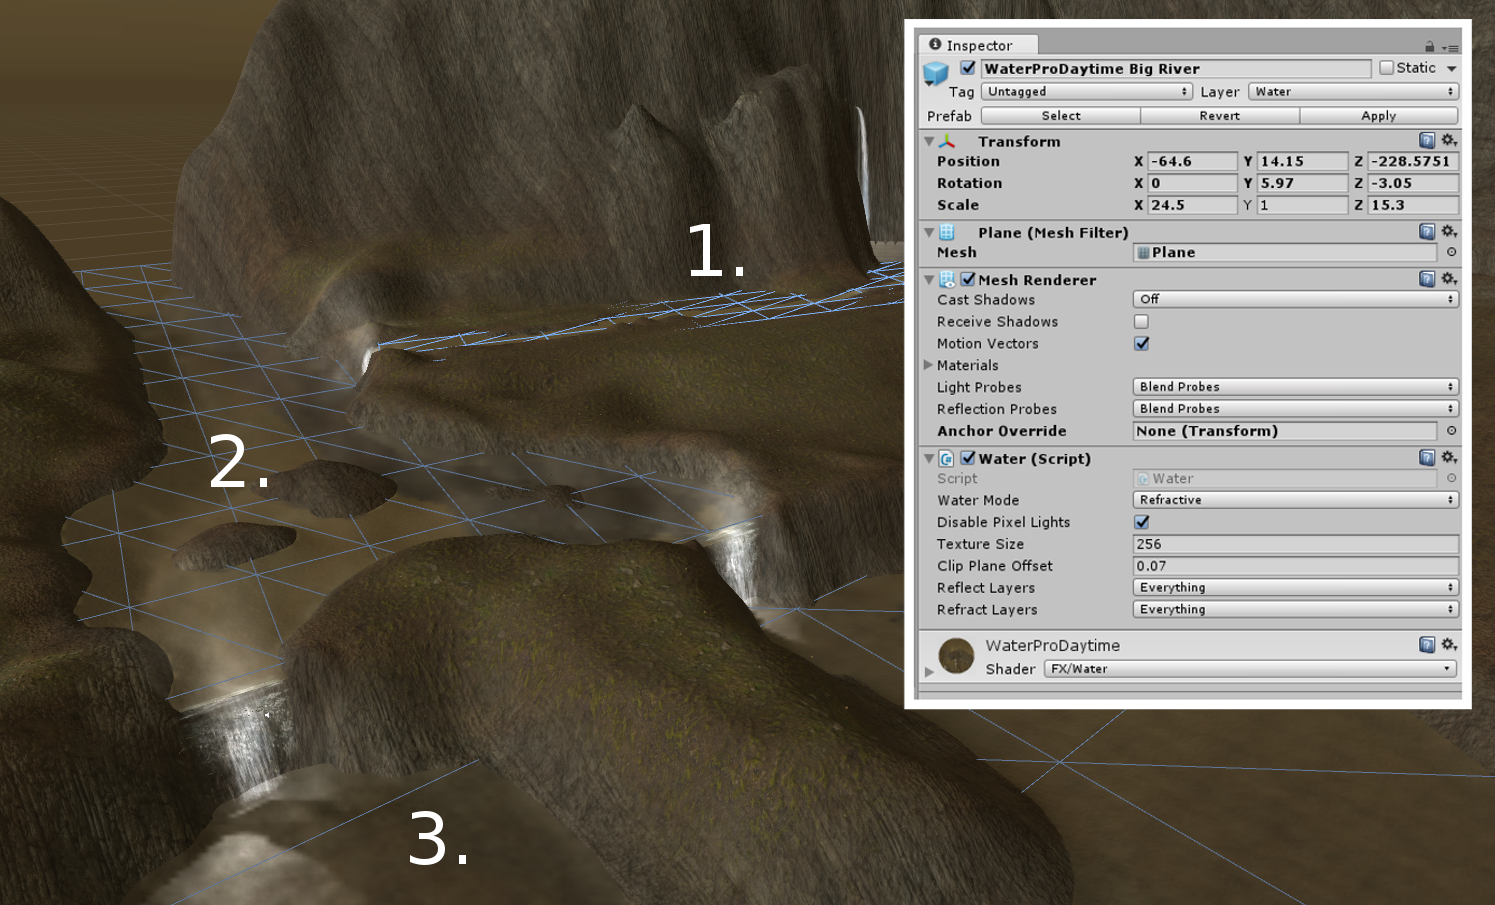
\includegraphics[width=0.95\linewidth]{Abbildungen/Unity/Water}
	\caption{Wasserebenen und exemplarische Einstellungen}
	\label{fig:Water}
\end{figure}

\subsubsection{Wasserfälle}
\begin{wrapfigure}{r}{0.5\textwidth}
	%\vspace{-20pt}
	\begin{center}
		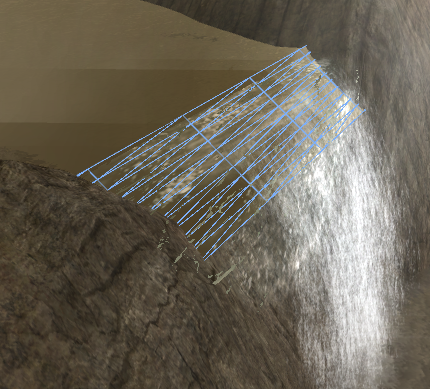
\includegraphics[width=0.45\textwidth]{Abbildungen/Unity/Waterfall}
	\end{center}
	\caption{Wasserfall}
	\label{fig:Waterfall}
\end{wrapfigure}

Trotz der Neigung der Flüsse konnten die Höhenunterschiede zwischen den Wasserebenen nicht ausgeglichen werden. Dadurch wurde es notwendig Wasserfälle in die Szene einzufügen. Diese stammen aus dem Assetstore und wurden für die Zwecke des Projektes angepasst. Die Abb. \ref{fig:Waterfall} zeigt den Übergang zwischen dem kleinen und großen Fluss. Um den harten Wechsel von Wasserebene zu Wasserfall abzuschwächen, war es nötig eine kleine abgeschrägte Ebene passgenau einzufügen. Ebenso mussten die seitlichen Ränder mit dem Terrainwerkzeug verdeckt werden. Diese Technik wurde auch bei den beiden anderen Wasserfällen vom großen Fluss zum Ozean angewendet.

\subsection{Animationen}
\subsubsection{Unity Animationen}
\begin{figure}[h]
	\centering
	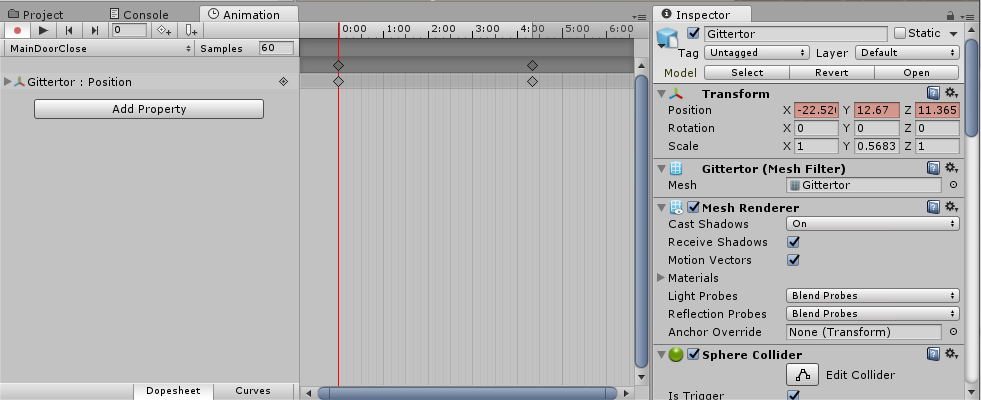
\includegraphics[width=0.95\linewidth]{Abbildungen/Unity/UnityAnim2}
	\caption{Erstellung von Animationen in Unity}
	\label{fig:unityAnim}
\end{figure}

Einfache Animationen, wie das Öffnen eines Burgtores können in Unity schnell und unkompliziert erstellt werden. In Abb. \ref{fig:unityAnim} ist das Werkzeug zur Erstellung von Animationen zu sehen. Im mittleren Teil sieht man die Keyframes und rechts die dazugehörigen \textit{Transform}-Werte. In unserem Fall des Burgtores wird das Schließen über zwei Keyframes mit unterschiedlichen Y-Werten definiert. Die so erstellten Animation stehen später im Animation Controller zur Verfügung.

\subsubsection{3d Studio Max Animation}

\begin{wrapfigure}{r}{0.6\textwidth}
	%\vspace{-20pt}
	\begin{center}
		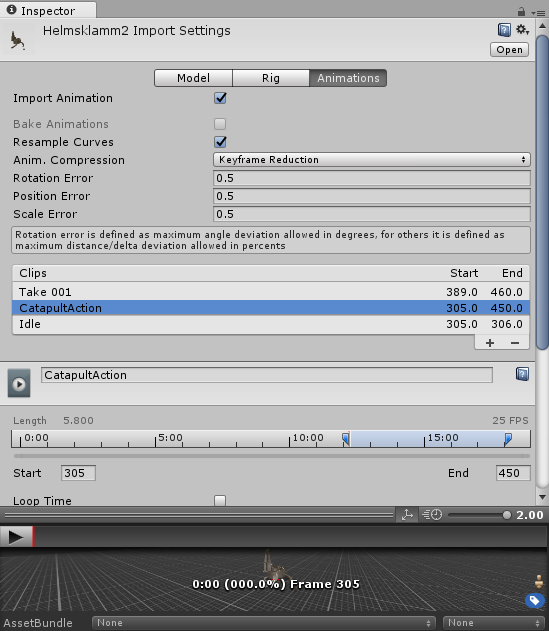
\includegraphics[width=0.55\textwidth]{Abbildungen/Unity/3dsAnim}
	\end{center}
	\caption{Animation aus 3d Studio Max}
	\label{fig:3dsAnim}
\end{wrapfigure}

Kommen die Animationen eines Modells aus 3d Studio Max liegen diese in einer Animationsspur im importierten Asset vor. Durch die Auswahl des Assets in der Assetübersicht können die einzelnen Animationen aus der gemeinsamem Spur extrahiert werden. In Abb. \ref{fig:3dsAnim} ist das benötigte Werkzeug zu sehen. Für unser Hauptmodell sieht man Beispielsweise die Zerstörungsanimation, die in den Keyframes 305 bis 450 vorliegt. Über die Plus-Schaltfläche können auch andere Animationen selektiert werden. Die auf diese Weise extrahierten Einzelanimationen stehen auf die gleiche Art und Weise, wie die in Unity erstellten zur Verfügung.  

\subsubsection{Animation Controller}

Der Animation Controller ist der bevorzugte Weg um Animationen zu kontrollieren und sie abzuspielen. Es handelt sich darin um einen Zustandsautomaten. In jedem Zustand wird eine Animation abgespielt. Übergänge von einem zum anderen bewirkt das Abspielen einer neuen Bewegung. Die Übergänge zwischen zwei Zuständen können mit Bedingungen versehen werden. In Abb. \ref{fig:animController} sieht man den Controller für das Burgtor. Zu Beginn der Szene wird in den \textit{MainDoorClosed} Zustand gewechselt. In diesem wird eine Ruhe-Animation abgespielt, welche dem geschlossenen Tor entspricht. Per Skript kann die Variable \textit{open} gesetzt werden und es erfolgt der Wechsel in den Zustand \textit{MainDoorOpen} der die Animation zum Öffnen des Tores abspielt. Ist diese beendet, wechselt der Automat in den Ruhe-Zustand des geöffneten Burgtores. Von diesem Zustand aus, kann über das Setzen der Variable \textit{close}, zum geschlossenen gewechselt werden. Über den Controller können auch Überblendungen zwischen den Animationen eingestellt werden. Die Einstellung dafür sind auf der rechten Seite der Abbildung zu sehen. So wird es möglich auch zwei Animationen nahtlos ineinander übergehen zu lassen. 


\begin{figure}[h]
	\centering
	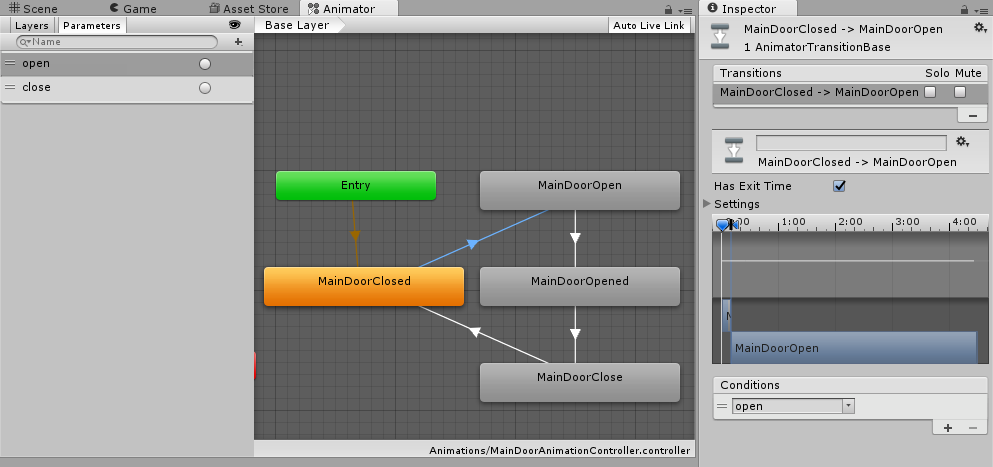
\includegraphics[width=0.95\linewidth]{Abbildungen/Unity/AnimationController}
	\caption{Animation-Controller zur Steuerung von Animationen}
	\label{fig:animController}
\end{figure}

\newpage
\subsection{Partikelsystem Fackel}
In wenigen Schritten und mithilfe des Partikelsystems in Unity kann man in kürzester Zeit schöne Feuereffekte erstellen.

\begin{figure}[H]
\centering
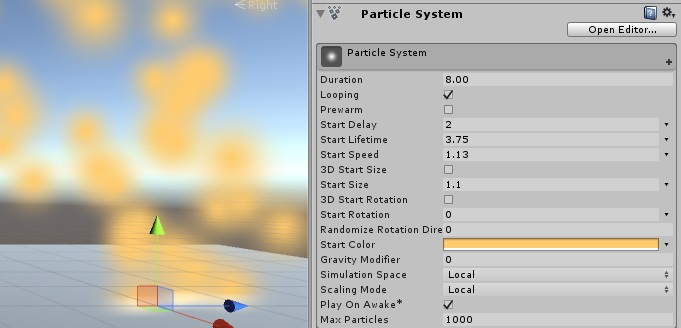
\includegraphics[width=0.95\linewidth]{Abbildungen/Unity/Fire/fire1}
\caption{Grundeinstellung Partikelsystem}
\label{fig:fire1}
\end{figure}

Im ersten Schritt wird ein Gameobject \textit{Particle System} erstellt und die in Abb. \ref{fig:fire1} abgebildeten Grundeinstellungen vorgenommen.

\begin{figure}[h!]
\centering
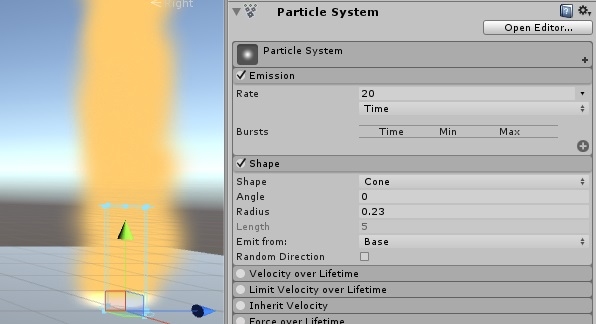
\includegraphics[width=0.95\linewidth]{Abbildungen/Unity/Fire/fire2}
\caption{Einstellungen Emission und Shape}
\label{fig:fire2}
\end{figure}

Um die Partikel zu verdichten und die horizontale Streuung einzugrenzen, wird die Emission erhöht und die Form angepasst. (siehe Abb.\ref{fig:fire2}) 

\begin{figure}[h!]
\centering
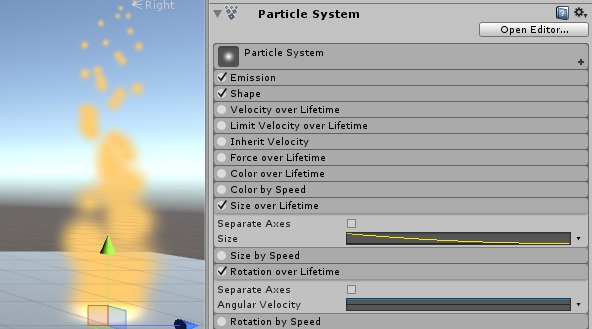
\includegraphics[width=0.95\linewidth]{Abbildungen/Unity/Fire/fire3}
\caption{Einstellungen Size over Livetime und Rotation over Lifetime}
\label{fig:fire3}
\end{figure}

Die typische Flammenform erreicht man, indem man die Größe im Bezug zur Lebensdauer anpasst. Dazu wählt man eine exponentiell sinkende Kurve. Außerdem versetzt man die Partikel in eine Rotation. (siehe Abb. \ref{fig:fire3})

\begin{figure}[h!]
\centering
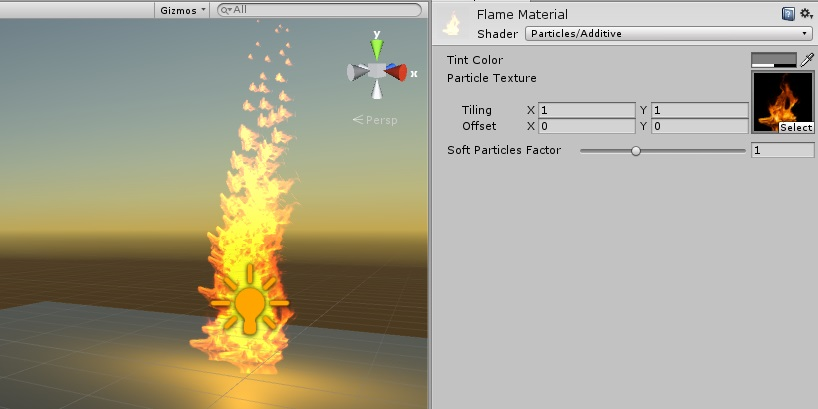
\includegraphics[width=0.95\linewidth]{Abbildungen/Unity/Fire/fire4}
\caption{Material und Point Light}
\label{fig:fire4}
\end{figure}

Um einen Flammenähnlichen Farbverlauf zu erreichen, muss man dem Partikelsystem ein Material zufügen. Dieses besteht aus dem Bild einer Flame auf schwarzem Hintergrund und entfaltet durch den Shader \textit{Particles/Additive} den gewünschten Effekt.

\newpage

\subsection{Benutzeroberfläche}

\begin{figure}[h]
	\centering
	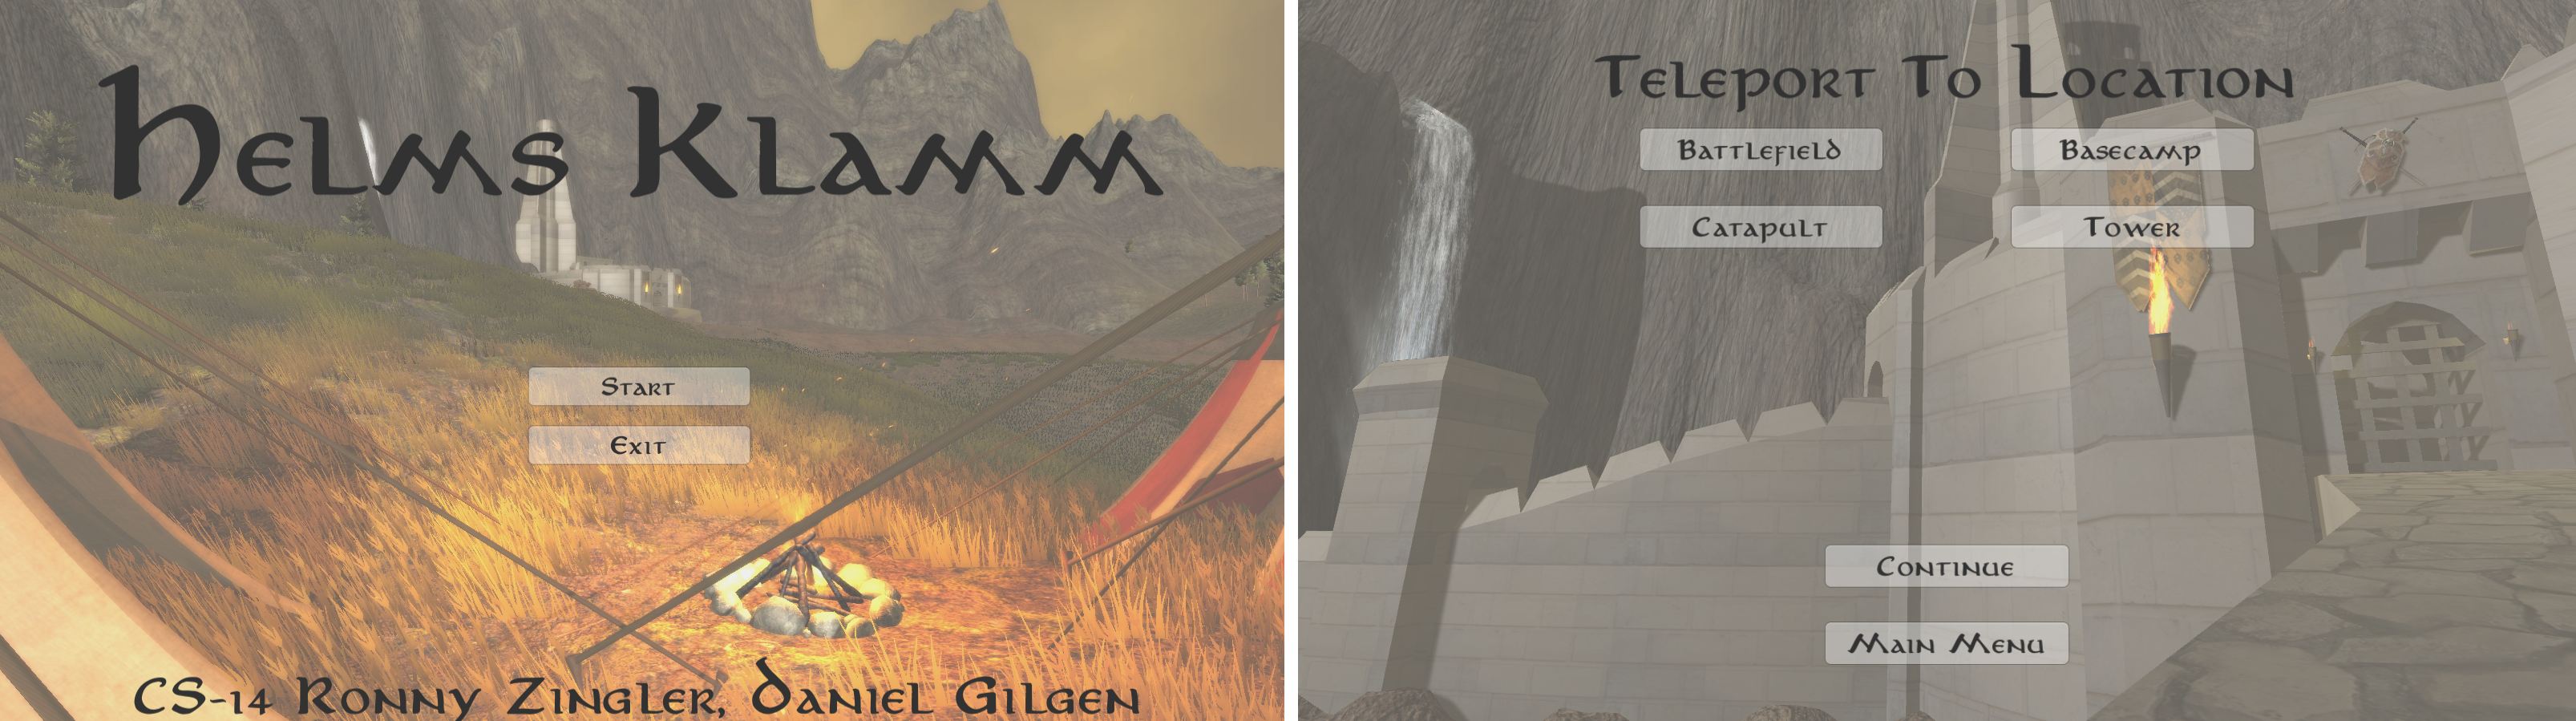
\includegraphics[width=0.95\linewidth]{Abbildungen/Unity/GuiCombined}
	\caption{Graphische Nutzeroberflächen}
	\label{fig:GuiCombined}
\end{figure}

%\begin{figure}[h]
%	\centering
%	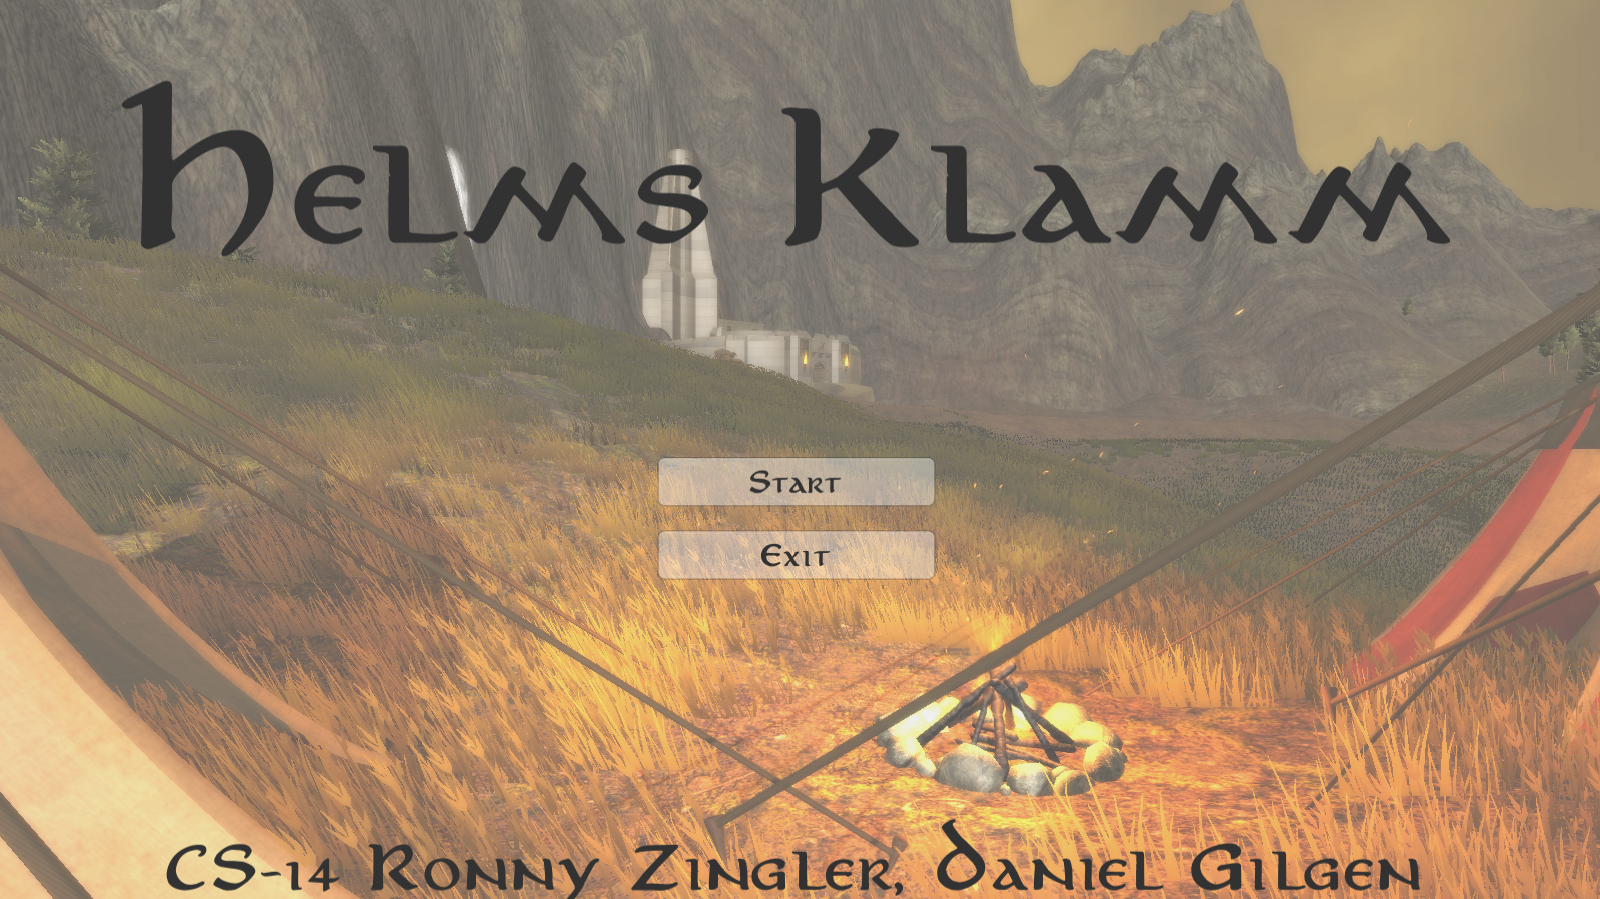
\includegraphics[width=0.95\linewidth]{Abbildungen/Unity/MainMenu}
%	\caption{Hauptmenü}
%	\label{fig:mainMenu}
%\end{figure}
%
%\begin{figure}[H]
%	\centering
%	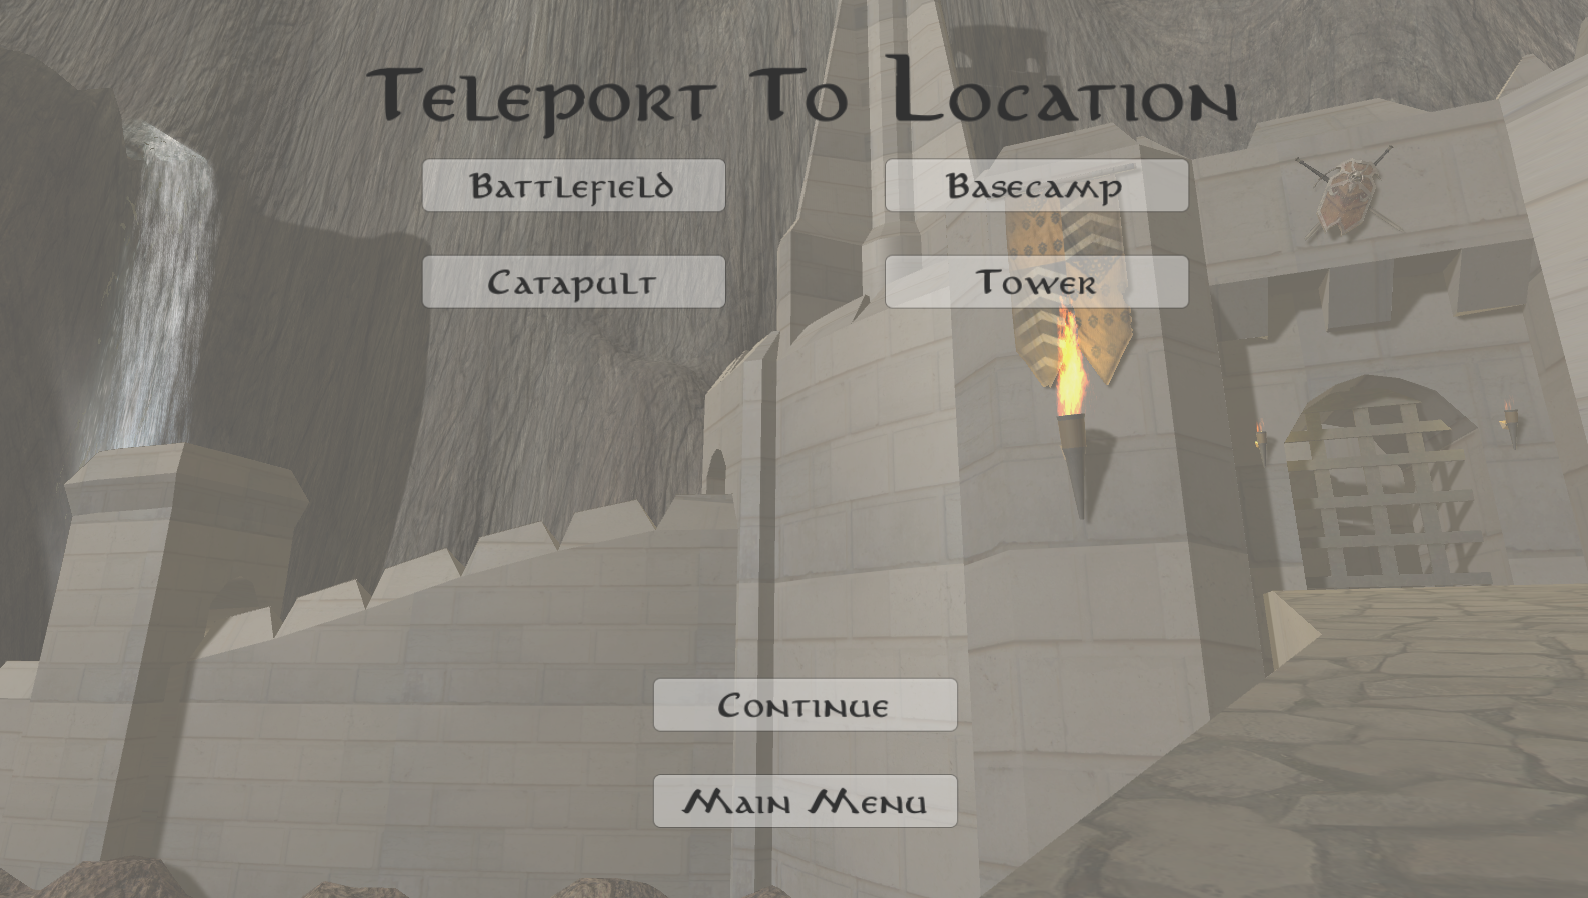
\includegraphics[width=0.95\linewidth]{Abbildungen/Unity/IngameMenu}
%	\caption{Spielmenü}
%	\label{fig:ingameMenü}
%\end{figure}

%\begin{wrapfigure}{r}{0.6\textwidth}
%
%	\begin{center}
%		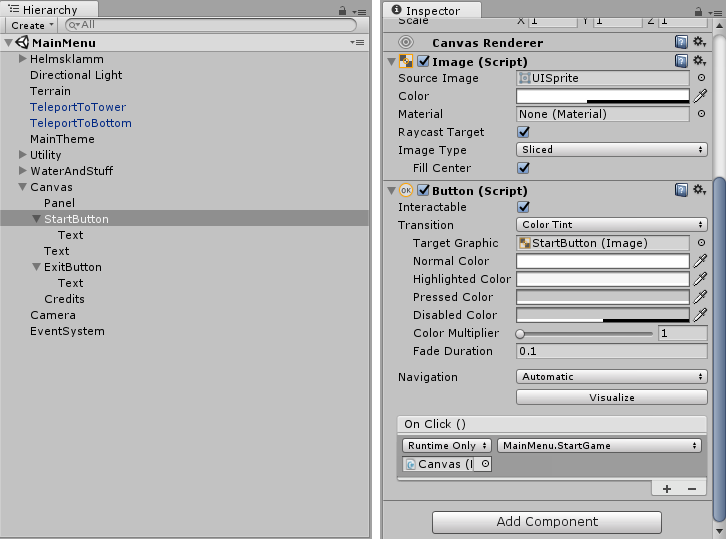
\includegraphics[width=0.55\textwidth]{Abbildungen/Unity/GuiExample}
%	\end{center}
%	\caption{Hierarchie und Inspektor für Startbutton}
%	\label{fig:3dsAnim}
%\end{wrapfigure}

\begin{figure}[h]
	\centering
	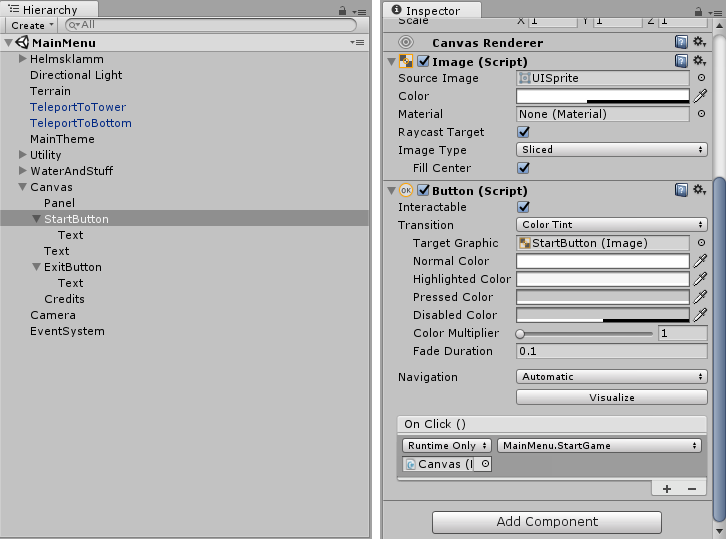
\includegraphics[width=0.95\linewidth]{Abbildungen/Unity/GuiExample}
	\caption{Hierarchie und Inspektor für Startbutton}
	\label{fig:GuiExample}
\end{figure}

Zur Erstellung von graphischen Nutzeroberflächen stehen in Unity vergleichbare Elemente wie in gängigen Programmiersprachen zur Verfügung. Grundelement einer jeden Benutzeroberfläche sind die \textit{Canvas}. In diese werden die Elemente über den Editor eingefügt, positioniert und individualisiert.  Es gibt verschiedene Möglichkeiten zur Darstellung. Für diesen Anwendungsfall wurde die Darstellungsart \textit{Screen Space - Overlay} gewählt. Dadurch werden die Elemente der Benutzeroberfläche bildschirmfüllend über die Szene gelegt. In Abbildung \ref{fig:GuiCombined} sieht man links das Haupt- und rechts das Spielmenü. Der generelle Aufbau beider Oberflächen ist sehr ähnlich. In Abb. \ref{fig:GuiExample} ist der Szenengraph des Hauptmenüs und die exemplarischen Einstellungen des Start-Buttons zu sehen. Die Szene des Hauptmenüs wurde von der eigentlichen abgeleitet. Unterschied ist die feste Kamera anstatt des \textit{FPS-Controllers} und die Entfernung jeglicher Umgebungsgeräusche. Stattdessen wird während der Darstellung des Hauptmenüs eine eingängige Musik abgespielt. Unten rechts in Abb. \ref{fig:GuiExample} ist zu sehen was beim Klicken des Start-Button erfolgt. In unserem Fall wird dadurch in die eigentliche Spielszene gewechselt.

\subsection{Audio}

\begin{wrapfigure}{r}{0.5\textwidth}
	\vspace{-20pt}
	\begin{center}
		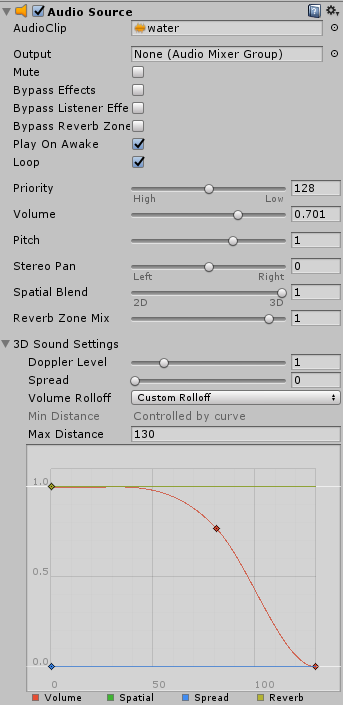
\includegraphics[width=0.45\textwidth]{Abbildungen/Unity/calmWaterAudio}
	\end{center}
	\caption{Audioeinstellungen}
	\label{fig:audioExample}
\end{wrapfigure}

Audioquellen können auf die gleiche Art und Weise wie 3d Objekte in der Welt platziert werden. Um diese zu hören, muss auf einem anderen Objekt ein \textit{Audio Listener} vorhanden sein. Im Fall unseres Projektes macht es nur Sinn, diesen bei einer Kamera oder dem Charakter zu platzieren. Das Platzieren zweier \textit{Listener} zur gleichen Zeit muss unbedingt vermieden werden. Abb. \ref{fig:audioExample} zeigt die Einstellungen der Wasserhintergrundgeräusche. Im oberen Teil ist sichtbar, dass die Geräusche sofort zum Beginn der Szene abgespielt werden und danach, bis zum Schließen dieser, wiederholt wird. Es ist natürlich ebenso möglich, Musik oder Tonquellen programmatisch zu starten. Im unteren Teil sind die Einstellungen zum Zusammenhang zwischen Entfernung und Lautstärke zu sehen. Im Falle des Wassergeräusches wurde eine eigene Kurve gewählt. Der Grund für diese Entscheidung, war das Vorhandensein zwei Tonquellen mit dem gleichen Geräusch. Nur dadurch war ein zufriedenstellendes Ergebnis für das plätschernde Geräusch des Wassers zu erreichen. Normalerweise genügen aber die beiden vordefinierten Lautstärke Kurven, logarithmisch und linear. Damit die \textit{3D Sound Settings} wirken, darf der Regler \textit{Spatial Blend} nicht auf 2D eingestellt werden.




 


\newpage
\section{Modellierung der Burg}

\subsection{Grundaufbau der Burg}

Als die Vorüberlegungen abgeschlossen waren, musste möglichst schnell ein grundlegendes Modell der Burg geschaffen werden. Dieses Modell sollte alle überlegten Maße einhalten und somit als Erstfassung dienen, um in eine Unity Szene eingefügt werden zu können.

\begin{figure}[h]
	\centering
	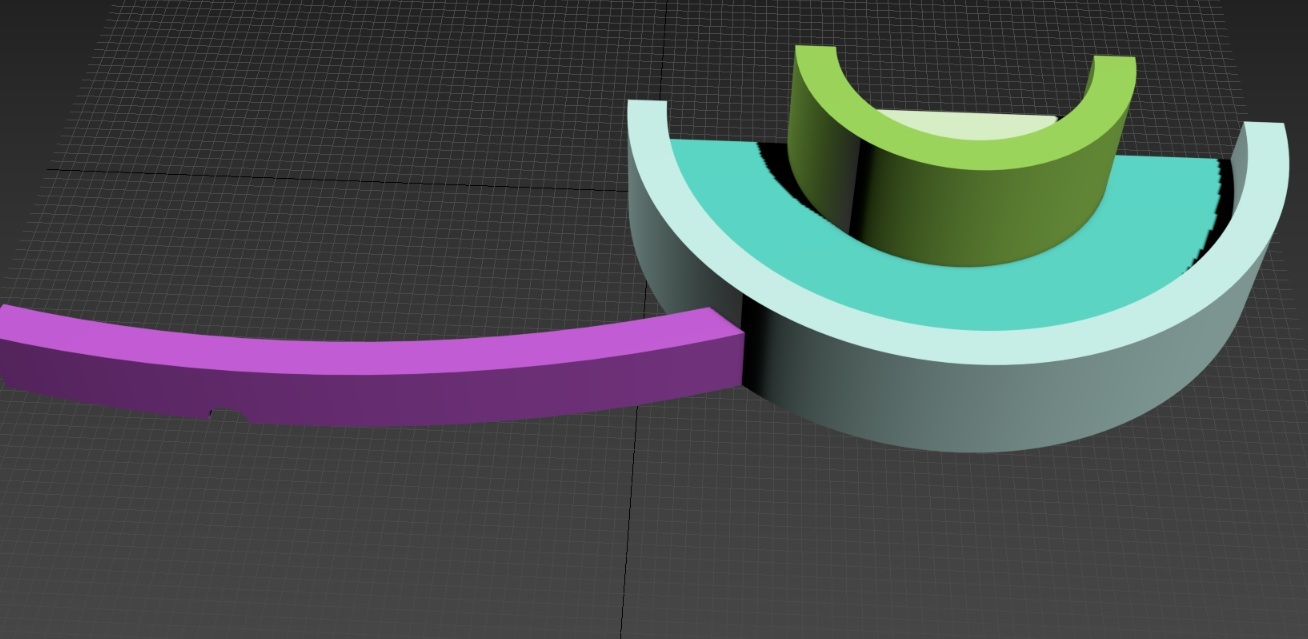
\includegraphics[width=0.95 \linewidth]{Abbildungen/3dsMax/Grundmodell}
	\caption{Grundaufbau der Burg}
	\label{fig:Grundaufbau}
\end{figure}

\begin{wrapfigure}{r}{0.5\textwidth}
	\begin{center}
		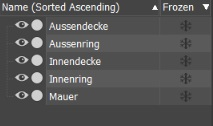
\includegraphics[width=0.45\textwidth]{Abbildungen/3dsMax/Grundhierachie}
	\end{center}
	\caption{Grundobjekte}
	\label{fig:Grundobjekte}
\end{wrapfigure}

Wie in den Abbildungen \ref{fig:Grundaufbau} und \ref{fig:Grundobjekte} zu sehen, besteht die Burg aus 5 Grundobjekten. Die Mauern wurden durch Röhren und die Decken durch Zylinder realisiert. Diese Objekte wurden anschließend in bearbeitbare Polys umgewandelt und zugeschnitten. Zum verschließen der daraus resultierenden offenen Enden wurde das Werkzeug \textit{Bridge} verwendet. Um später einen Fluss durch die lange Mauer fließen zu lassen, wurde unter Zuhilfenahme eines Zylinders und der boolschen Operation Subtrahieren eine halbrunde Öffnung hinzugefügt.

\newpage
\subsection{Modellierung des Haupttors}

\begin{figure}[h]
	\centering
	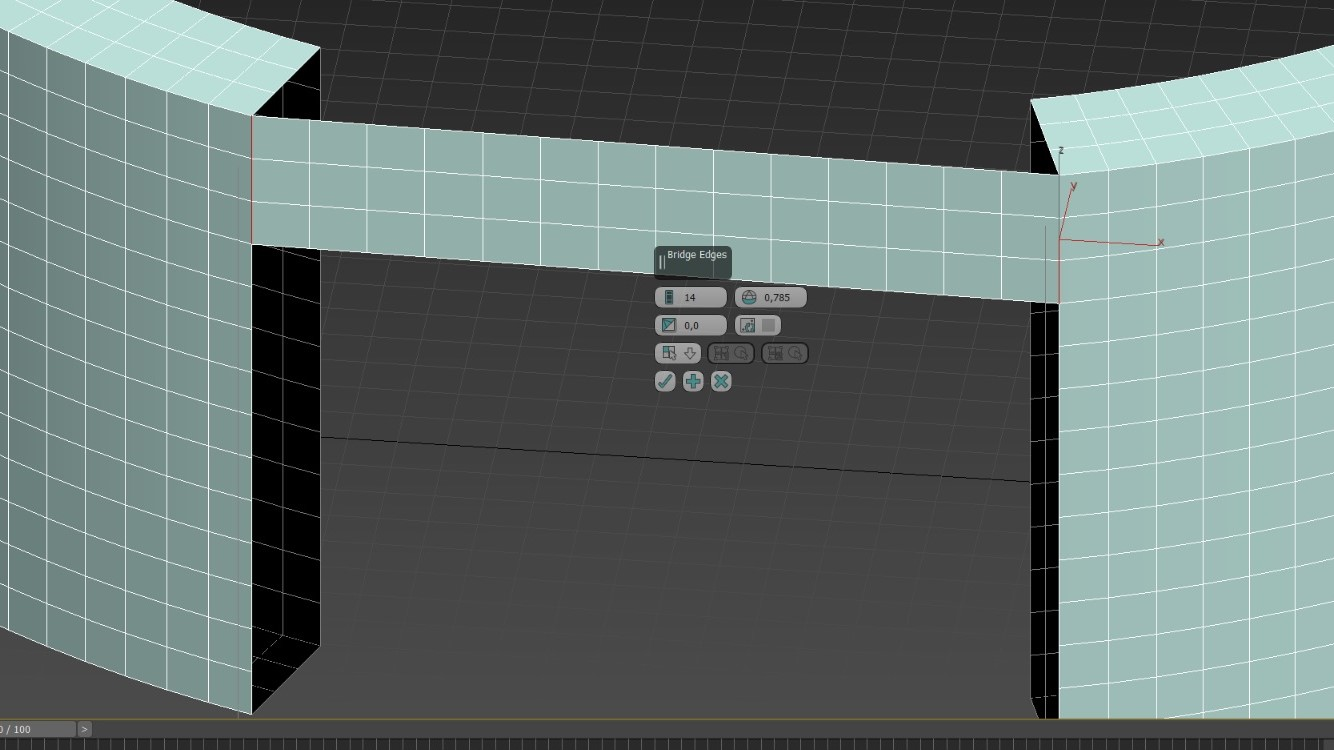
\includegraphics[width=0.95 \linewidth]{Abbildungen/3dsMax/Haupttor}
	\caption{Vorarbeit Haupttor}
	\label{fig:Haupttor}
\end{figure}

\begin{wrapfigure}{r}{0.5\textwidth}
	\begin{center}
		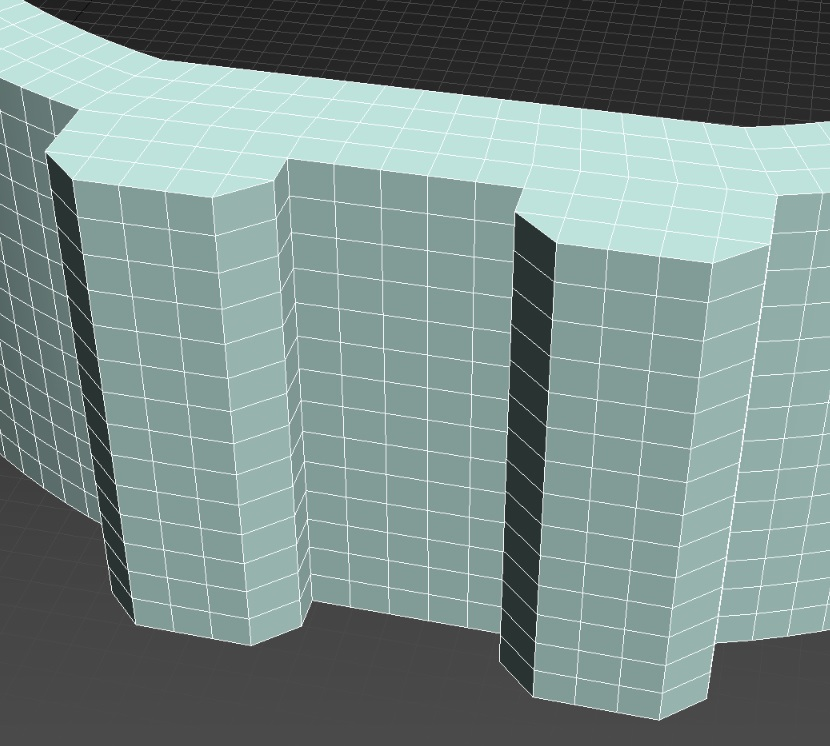
\includegraphics[width=0.45\textwidth]{Abbildungen/3dsMax/Haupttor2}
	\end{center}
	\caption{Haupttor}
	\label{fig:Haupttor2}
\end{wrapfigure}



Der nächste Schritt umfasste die Modellierung des Haupttores. Um eine gerade Arbeitsfläche zu erhalten, wurde der Mittelteil des Außenrings herausgeschnitten. Die nun freilegenden Kanten wurden, wie in Abb. \ref{fig:Haupttor} zu sehen mit dem \textit{Bridge} Werkzeug verbunden. Die Türme des Tores wurden anschließend mit dem \textit{Extrude} Werkzeug herausgearbeitet. Wie in Abb. \ref{fig:Haupttor2} zu sehen sind die frontalen Ecken der Türme "abgeschnitten". Um dies zu erreichen gibt es in 3dsMax verschiedene Möglichkeiten. In diesem Fall wurde das Kantenwerkzeug \textit{Chamfer} benutzt. Dies erlaubt es Ecken durch automatisches hinzufügen neuer Kanten abzurunden. Um das gewünschte Ziel zu erreichen wurde die Kantenanzahl verdoppelt.

\newpage
\subsection{Treppenbau}

\begin{figure}[h]
	\centering
	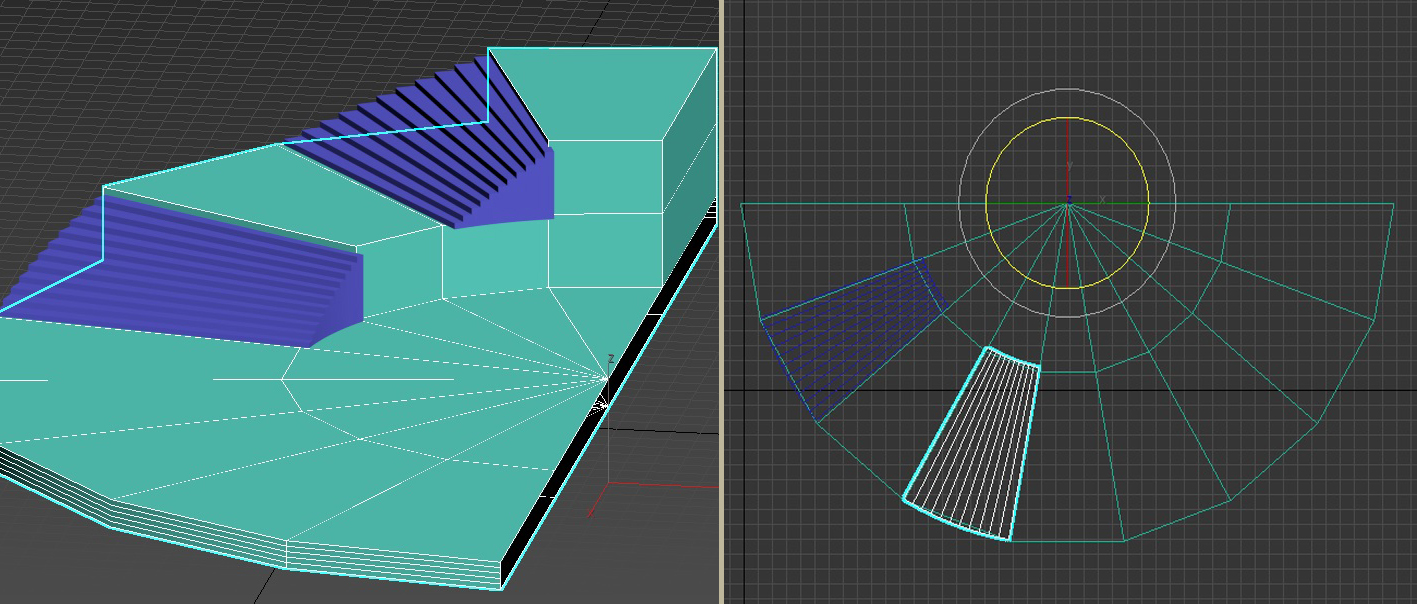
\includegraphics[width=0.95 \linewidth]{Abbildungen/3dsMax/Treppe_final}
	\caption{Treppenbau}
	\label{fig:Treppe}
\end{figure}

\begin{wrapfigure}{r}{0.3\textwidth}
	\begin{center}
		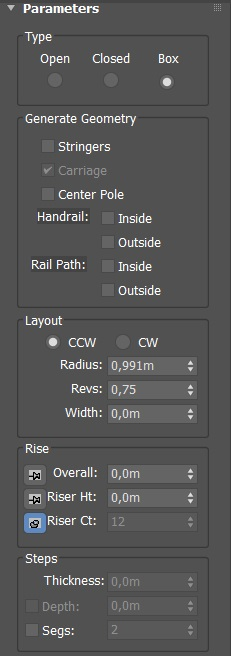
\includegraphics[width=0.25\textwidth]{Abbildungen/3dsMax/Treppe3}
	\end{center}
	\caption{Treppenparameter}
	\label{fig:Parameter}
\end{wrapfigure}

Um den erhöhten Innenring zu erreichen, musste eine Möglichkeit gefunden werden den Höhenunterschied auszugleichen. Treppen waren das Mittel der Wahl. Dazu wurde, wie in Abb. \ref{fig:Treppe} links zu sehen, die Außendecke mit dem\textit{Extrude} Befehl angepasst. Über die 3dsMax Objektauswahl können direkt Treppen als Grundobjekte erstellt werden. Da die Treppen in eine Rundung eingepasst werden sollten, wurden die \textit{SpiralStairs} gewählt. Abb. \ref{fig:Parameter} zeigt einen Ausschnitt der zu modifizierenden Parameter. Um einen geschlossenen Treppenkörper zu erhalten, wurde \textit(Box) gewählt. Der Radius der Treppe gleicht dem der Außendecke, um eine genaue Einpassung zu ermöglichen. Die Treppe wurde nun , wie in Abb. \ref{fig:Treppe} rechts gesehen, so verschoben, dass der Pivot Punkt der Treppe, dem der Außendecke entspricht. Um Sicherzustellen das später der First Person Controller die Treppen erklimmen kann, wurde darauf geachtet, dass Stufenhöhe und -tiefe Maßen entsprechen, welche auch in der Realität Anwendung finden. Dies ermöglichte der Parameter \textit{Riser Ht}, der zwischen 20cm - 30cm gewählt wurde. Auch im weiteren Modellierungsprozess wurden vermehrt Treppen eingesetzt, um die Begehung der Burg spannender zu gestalten.

\newpage
\subsection{Verfeinerung der Mauern}

\begin{figure}[h]
	\centering
	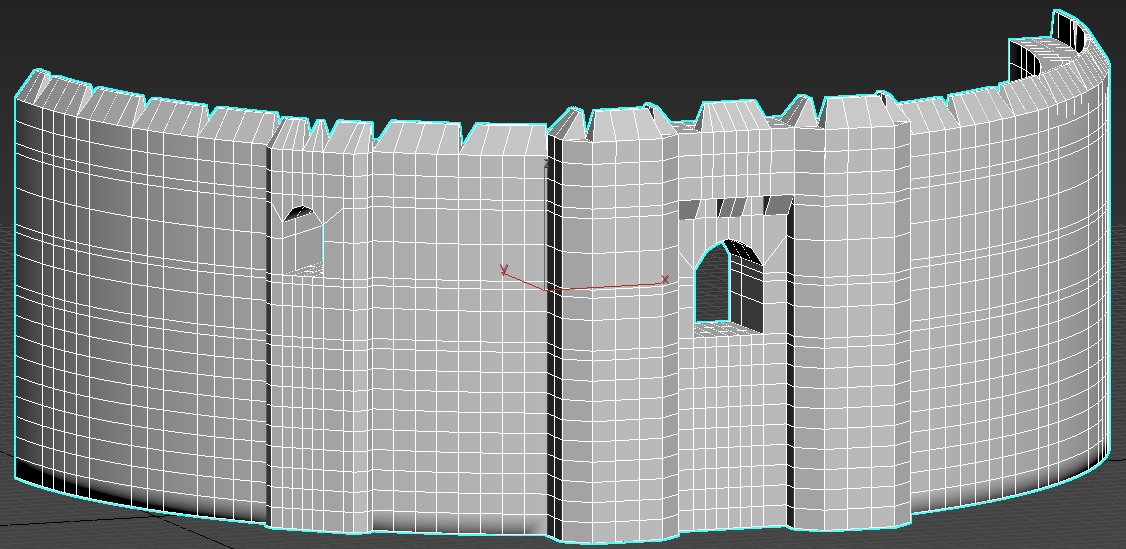
\includegraphics[width=0.95 \linewidth]{Abbildungen/3dsMax/Aussenring}
	\caption{Verfeinerung Außenring}
	\label{fig:Aussenring}
\end{figure}

Um den Außenring detaillierter zu gestalten, wurden hauptsächlich die Polygonwerkzeuge \textit{Extrude} und \textit{Bevel} genutzt. Durch paarweises auswählen und \textit{Bevel} wurden die Zinnen herausgearbeitet. Auch die obere Seite des Haupttores wurde mittels \textit{Extrude} detaillierter gestaltet. Um die Toröffnung herauszuarbeiten, wurden mithilfe des Kantenauswahlwerkzeugs \textit{Ring} alle horizontalen Kanten ausgewählt und mittels \textit{Connect} neue vertikale Kanten eingefügt. Durch gezieltes verschieben von Eckpunkten wurde die obere Rundung geforrmt. Der Durchgang wurde durch löschen der Polygone geschaffen und die daraus resultierenden offenen Fläche mithilfe des \textit{Bridge} Werkzeugs geschlossen. 

\begin{figure}[h]
	\centering
	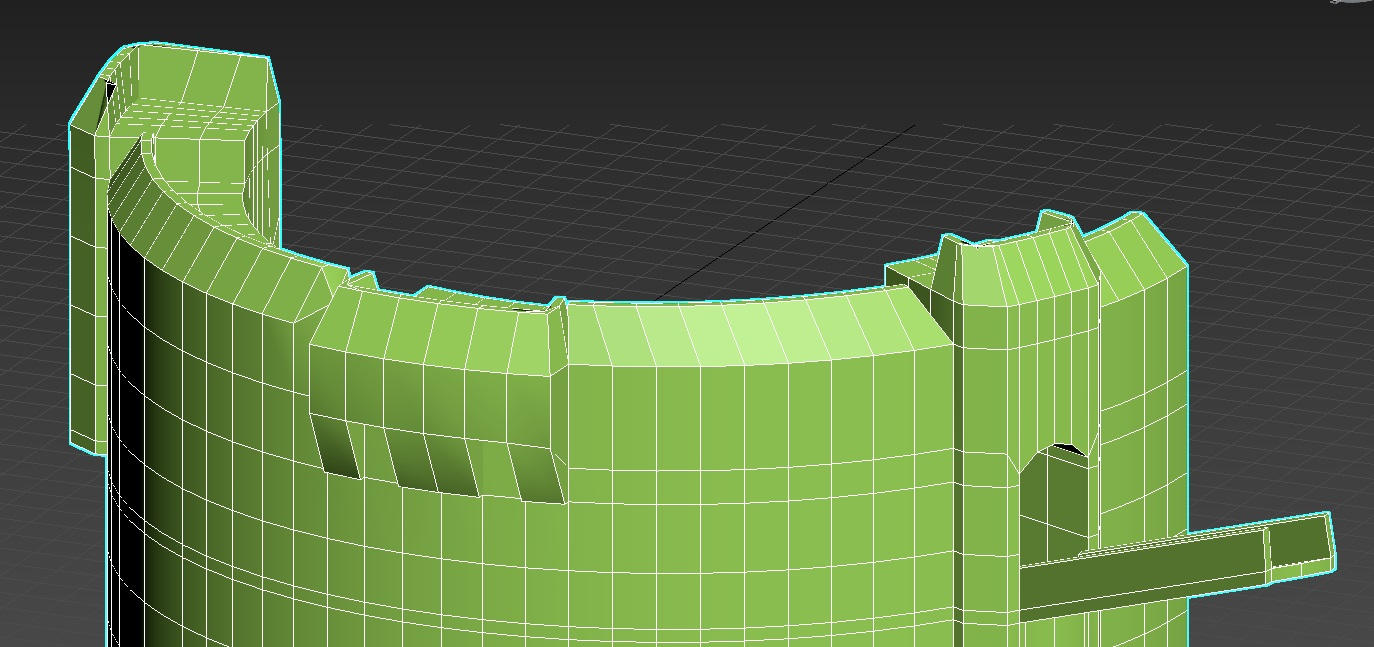
\includegraphics[width=0.95 \linewidth]{Abbildungen/3dsMax/Innenring}
	\caption{Verfeinerung Innenring}
	\label{fig:Innenring}
\end{figure}

Wie in Abb. \ref{fig:Innenring} zu sehen, wurde der Innenring ähnlich zum Außenring gestaltet, um einen einheitlichen Gesamteindruck zu erhalten. Die Zinnen sind aber ohne Schießscharten gehalten. Zum Abschluss wurde noch durch den \textit{Extrude} Befehl eine Brücke zum erreichen des Außenrings angefügt.

\begin{figure}[h]
	\centering
	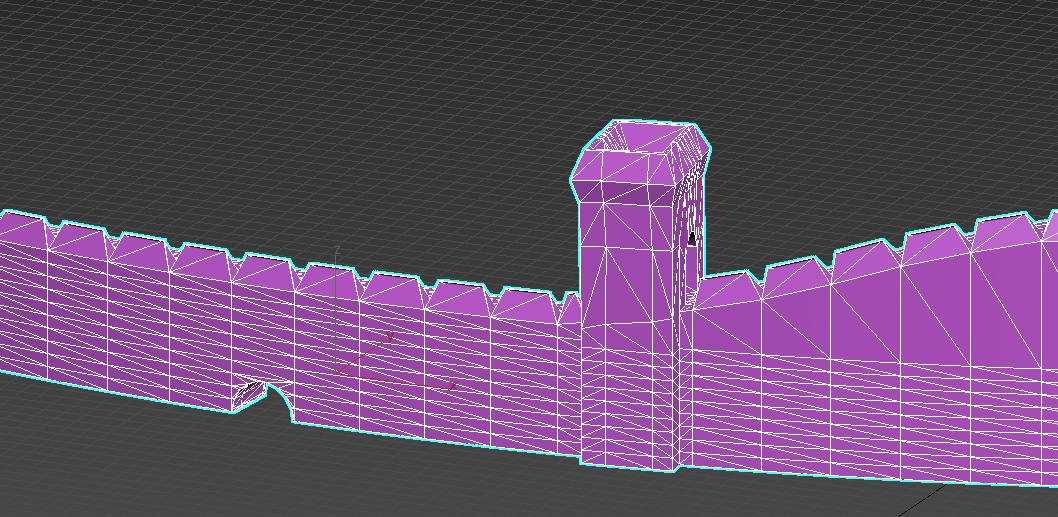
\includegraphics[width=0.95 \linewidth]{Abbildungen/3dsMax/Mauer}
	\caption{Verfeinerung Mauer}
	\label{fig:Mauer}
\end{figure}

Abb. \ref{fig:Mauer} zeigt die lange Verteidigungsmauer und den bereits erwähnten Flussdurchgang. Auch hier wurden Zinnen herausgearbeitet und des weiteren ein Wachturm mit Durchgang angefügt.
\newpage

\subsection{Haupthaus und Turm}

\begin{figure}[h]
	\centering
	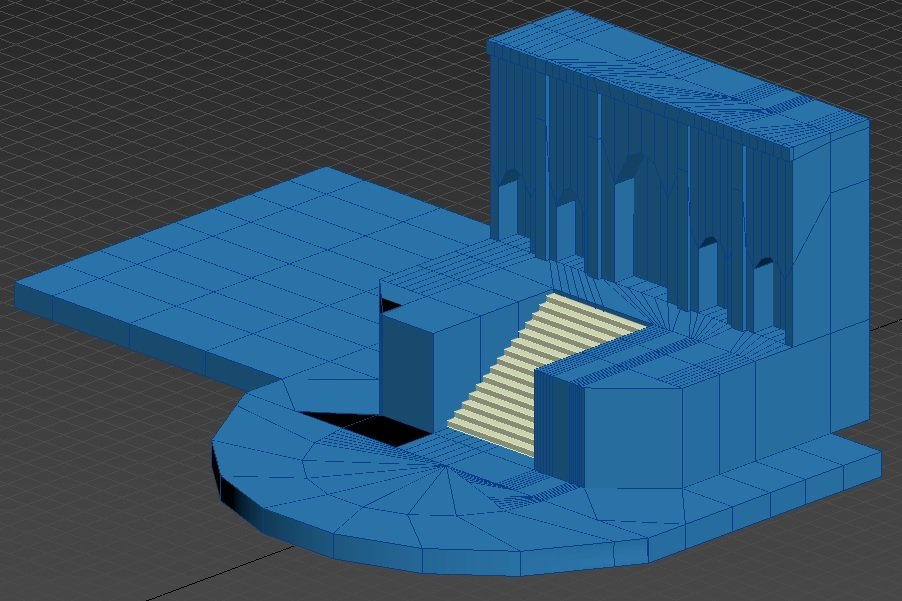
\includegraphics[width=0.95 \linewidth]{Abbildungen/3dsMax/Gebaeude}
	\caption{Haupthaus}
	\label{fig:Haupthaus}
\end{figure}

\begin{wrapfigure}{r}{0.3\textwidth}
	\begin{center}
		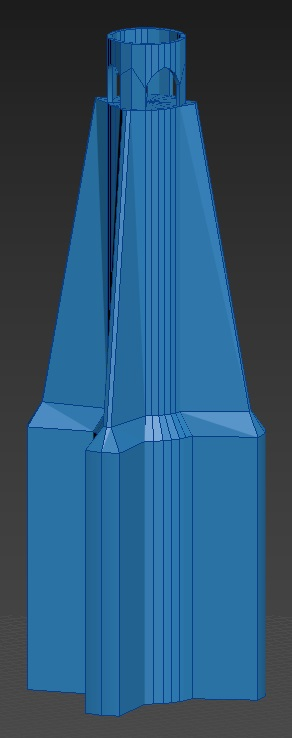
\includegraphics[width=0.22\textwidth]{Abbildungen/3dsMax/Turm}
	\end{center}
	\caption{Turm}
	\label{fig:Turm}
\end{wrapfigure}

Um Platz für das in Abb. \ref{fig:Haupthaus} zu sehende Haupthaus zu schaffen, wurde die halbrunde Innendecke mit mehrfachem Einsatz des \textit{Extrude} Befehls erweitert. Auch eine Plattform für den in Abb. \ref{fig:Turm} zu sehenden Turm wurde geschaffen. Der Turm besteht aus einem Zylinder, welcher durch das \textit{Extrude} und \textit{Bevel} Werkzeug in die gewünschte Form gebracht wurde. Ähnlich der Durchgänge, wurden Aussparungen am oberen Teil des Turmes angebracht.
\newpage

\subsection{Texturierung der Burg}

\begin{figure}[h]
	\centering
	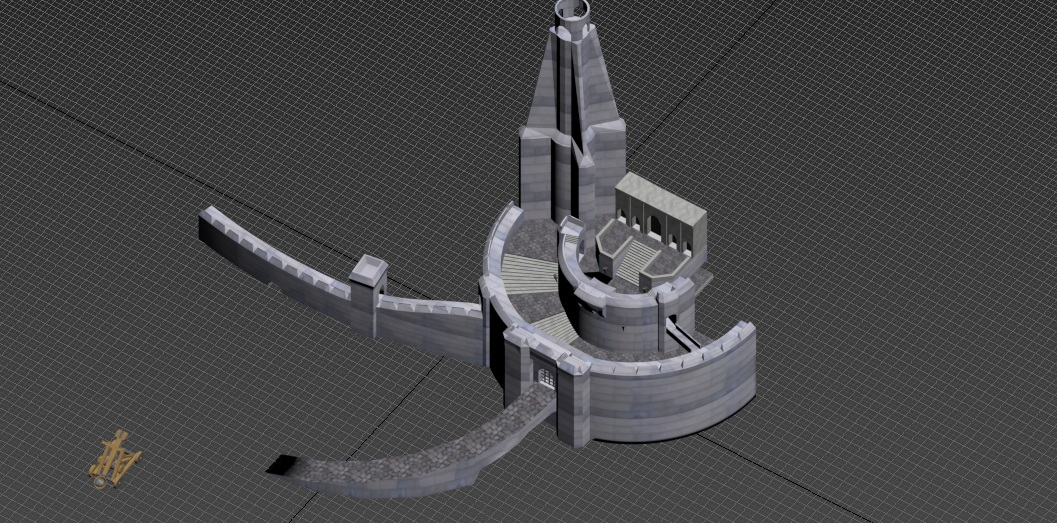
\includegraphics[width=0.95 \linewidth]{Abbildungen/3dsMax/Burg_final}
	\caption{texturierte Burg}
	\label{fig:Burg_final}
\end{figure}
 
\newpage
\section{Skripte}
\subsection{Allgemein}
Im zu bearbeitenden Projekt wurde die C-Sharp als Programmiersprache ausgewählt. Gründe hierfür waren die statische Typisierung und die Ähnlichkeit zu Java. Der Einstieg in das Skripten der Szene stellte sich als anspruchsvoll heraus. Ohne eine grundlegendes Verständnis der verschiedene Einstiegspunkte in ein Skript, z. B. \textit{Update}, war es nicht möglich mit der Programmierung zu beginnen. Deshalb soll an dieser Stelle auf einige wichtige Erkenntnisse, für das Arbeiten mit Klassen, die von \textit{MonoBehaviour} erben, eingegangen werden.

\begin{itemize}
	\item \textbf{Öffentliche Variablen:} Mit \textit{public} gekennzeichnete Attribute können über den Editor per Drag and Drop belegt werden.
	\item \textbf{Suche nach Objekten:} Befindet sich das Skript in Objekt A, können Referenzen auf Unterobjekte von A per \textit{GetComponent<TYP>} angefordert werden. TYP kann beispielsweise \textit{AudioSource} sein. Liegen mehrere des gleichen Typs vor kann die Methode \textit{GetComponents<TYP>} benutzt werden. Sollen Referenzen auf beliebige Objekte in einer Szene gefunden werden bietet sich die statische Methode \textit{GameObject.Find("Name des Objekts")} an.
	\item \textbf{Aktualisierung eines Objektes:} Soll ein Objekt während des \textit{Renderns} aktualisiert werden, gibt es die Methode \textit{Update}. Diese wird bei jeder Berechnung eines \textit{Frames} aufgerufen. Dort können beispielsweise Transformationen oder andere Aktionen ausgelöst werden.
	\item \textbf{Initialisierung eines Objektes:} Für diesen Anwendungsfall existiert die Methode \textit{Start}. An dieser Stelle können beispielsweise Referenzen auf andere Objekte gesucht werden. Dadurch muss dies nicht bei jedem Aufruf der\textit{Update}-Methode geschehen.
	\item \textbf{Kollisionserkennung:} Gibt es am skriptenthaltenden Objekt ein \textit{Collider} so existieren die Methoden \textit{OnTriggerEnter} oder \textit{OnTriggerExit}. Über diese kann erkannt werden, wenn sich zum Beispiel der Spieler in die Nähe des Katapult begibt oder sich wieder entfernt.
\end{itemize}

Nach Erlangung, der für dieses Projekts wichtigsten Verständnisse, bestand die Programmierung der Szene weitgehend aus dem Lesen der Dokumentation und Anwendung dieser.

\subsection{Beispiel Innentür}
\lstinputlisting[caption=Öffnen der Innentür, label=lst:door.cs]{Skripte/Door.cs}

Im Codebeispiel \ref{lst:door.cs} soll auf das Öffnen der inneren Burgtor erklärt werden. Dieses Beispiel wurde gewählt, weil die Richtung zum Öffnen der Tür von der Position des Spieler abhängt. Zusätzlich werden verschiedene Sounds für das Öffnen und Schließen verwendet. In den Zeilen 5 bis 17 werden die verschiedenen Attribute der Klasse deklariert und teilweise initialisiert. Erwähnenswert sind die drei Hashes auf den Zeilen 13 bis 15. Diese dienen zum schnelleren Vergleich der Zustände des \textit{Animation Controllers}. In der Methode \textit{Start} werden die verschiedenen Attribute initialisiert. Wichtig für das weitere Verständnis ist das Attribut \textit{directionPlane}. Es handelt sich um ein Verweis auf eine Rechteck, welches plan auf der ungeöffneten Tür liegt. Durch dieses kann später berechnet werden auf welcher Seite  der Tür sich der Spieler befindet. Die beiden Funktionen auf den Zeilen 61 bis 77 setzen die Variable \textit{inRange} auf wahr oder falsch, je nach dem, ob sich der Spieler in der Reichtweite zur Tür befindet.

Die Methode \textit{Update} stellt die eigentliche Funktionalität zur Interaktion mit der Tür bereit. Zu Beginn wird geprüft, ob der Spieler sich in Reichweite der Tür befindet. Ist die nicht der Fall, wird die Methode sofort verlassen.
Anschließend wird abgefragt, ob die Taste E gedrückt wurde. Sollte dies eintreffen, wird der Vektor von Spieler zur Tür berechnet und der Normalvektor der \textit{directionPlane} ausgelesen. Zusätzlich wird der \textit{Animation Controller} nach seinem Zustand gefragt. Auf den Zeilen 41 und 53 wird über den Zustand des \textit{Animation Controllers} herausgefunden, ob die Tür gerade geschlossen oder offen ist. Wird in diesem Moment eine Öffnen- oder Schließen-Animation abgespielt wird dieser Block übersprungen. Falls sie geschlossen ist, wird auf Zeile 43 über den Winkel zwischen dem Vektor von Spieler zu Tür und dem Normalvektor herausgefunden, auf welcher Seite der Spieler sich befindet. Abhängig davon, wird über \textit(setTrigger) die Tür nach Innen oder Außen geöffnet und zusätzlich auf Zeile 52 das Geräusch zum Öffnen abgespielt. Ist die Tür offen, muss die Position des Spielers nicht beachtet werden und die Animation bzw. der Ton wird einfach abgespielt.  

Die anderen Skripte der Szene folgen diesen Mechanismen und können gerne im Rahmen der Präsentation besprochen werden.

  
 
\newpage 
 
% Abbildungsverzeichnis
\listoffigures
 \newpage
\end{document}
